\documentclass[11pt,a4paper]{article}
\usepackage[margin=2.5cm]{geometry}
\usepackage[T1]{fontenc}
\usepackage[utf8]{inputenc}
\usepackage{lmodern}
\usepackage{microtype}
\usepackage{amsmath}
\usepackage{graphicx}
\usepackage{booktabs}
\usepackage[font=small,labelfont=bf]{caption}
\captionsetup[table]{position=top}
\usepackage[section]{placeins} % keeps each figure within its own section
\usepackage{parskip}           % blank line between paragraphs, no indentation
\usepackage[round]{natbib}
\usepackage{xurl}
\usepackage{xcolor}
\usepackage[colorlinks=true, linkcolor=blue!50!black, citecolor=blue!50!black,
            urlcolor=blue!60!black]{hyperref}

\title{In-context graph learning in language models:\\
induction circuits, learning curves and scaling laws}
\author{Federico Viola}
\date{November 2026}

\begin{document}

\maketitle

\begin{abstract}
We reproduce and extend experiments on, and compare hypotheses about, the in-context learning of graph structure in
language models. The graph is presented as a random walk on it, in which each node is a single-token English word and
no semantic connection between the words is assumed; the model learns to predict the next word according to the graph
structure. Previous work has shown that the graph structure emerges in the hidden activations of the model, and has
provided evidence that induction circuits play a substantial role in the phenomenon. We give further evidence for the
role of induction circuits by separating the contributions of different types of attention heads at the final token
and in the preceding history of the walk. We also compare hypotheses about the learning curve of the model, and find
evidence for a smooth, sigmoid-like curve whose midpoint roughly follows a sublinear power law in the number of
vertices.

\medskip
\noindent\textbf{Code and results:} \url{https://github.com/federicov99/in-context-graph-learning}
\end{abstract}

\section{Introduction and previous work}

The phenomenon of in-context learning in language models (LMs), in which models learn and use information from their
context without changing their weights, provides evidence that models can adapt to situations entirely unseen in their
training data and develop capabilities related to the new context. However, the phenomenon is not yet fully
understood. Researchers have been investigating how models encode the new information in their internal activations,
which elements of their architecture contribute to the process, whether they can consistently build a world model from
the data seen in context, and whether they can flexibly use this structure when presented with novel tasks.

One simple setting in which in-context learning arises, studied in several recent works, presents the model with a
sequence of words generated by a random walk on a graph, in which each node corresponds to a single-token English word
and there is no built-in semantic connection between the words. \citet{park2025} showed that in this setting the model
learns the graph structure from the walk in its context: after a sufficiently long walk, it predicts a next word that
respects the adjacency of the graph with high accuracy. Moreover, as the walk progresses, the internal representations
of the words in a late layer arrange themselves in a structure that resembles the graph.

Subsequent works have replicated the experiment of Park et al.\ and asked which internal mechanisms build these
representations, whether the representations causally affect the predictions, and whether the model can use them for
other tasks. In particular, \citet{arditi2026} argued that the phenomenon can be explained by induction circuits
\citep{olsson2022}, a well-known attention mechanism in which some heads attend to the token immediately after an
earlier copy of the current token; this is made possible by heads in earlier layers that attend mainly to the previous
token and copy information about which token each token follows. \citet{kowalyshyn2026} fitted a belief model to the
accuracy curve of an experiment in which walks on two competing graphs are presented one after the other, and used
activation patching and steering to argue that the in-context representations learned from the walk (the activations
that follow the graph geometry) have a causal effect on the predictions. They concluded that neither induction circuits
nor structure inference alone suffices to explain in-context graph learning, and that the evidence is most consistent
with both mechanisms operating in parallel.

\citet{lepori2026} argued that the internal representations cannot be flexibly deployed in other contexts, and are
difficult for the model to use even in the same context at a later time. In their experiments, the next-token accuracy
falls when intermediate tokens separate the walk from the prediction, and on other tasks, such as identifying a word
two or three steps away in the graph, accuracy hardly rises above baseline: the learned representations do not allow
the model to perform adaptive world modeling. \citet{matsutani2026} then showed that accuracy on adaptive world
modeling can be improved by few-shot demonstrations, in which the model is shown a few examples of the same task
performed on graphs with different words.

We perform two experiments. In the first, we ablate induction and previous-token heads as in \citet{arditi2026}, but
distinguish between ablating them only at the last position and only in the preceding history. We find that
previous-token heads have a negligible effect at the last position (about 2 percentage points beyond a layer-matched
control for the top 32 heads, against about 51 in the history), while induction heads have comparable effects in the
two places (38 points at the last position and 40 in the history). In the second experiment, we fit the accuracy curve
with the belief model of \citet{kowalyshyn2026} across graph sizes. The belief curve describes the data well, and its
midpoint scales roughly as $N^* \approx 4.75\, n^{0.89}$ in the number of vertices $n$: about 1.6 to 2 times the
context at which the walk has shown half of each word's neighbours. This is consistent with the role of induction
circuits found in the first experiment.

\section{Experiment 1: ablations targeting induction circuits}

Our first experiment is a narrow extension of the head-ablation experiment of \citet{arditi2026}, which examines the
role of induction circuits \citep{olsson2022} in more detail. These circuits are composed of two types of attention
heads: \emph{previous-token heads}, which at a token $T$ attend to the token $P(T)$ immediately before it and can copy
information about $P(T)$ into the residual stream at $T$; and \emph{induction heads}, which use that information in a
later layer: when a copy of $P(T)$ appears later in the context, they attend from it to $T$ and help predict $T$ as the
next token. Both types of heads can be identified by running the model on a sequence of random tokens repeated twice
\citep{olsson2022}.

As in \citet{arditi2026}, we identify the previous-token and induction heads of the model (an open-weight model of the
Llama, Qwen or Mistral family, with 1B to 15B parameters) by ranking them according to how strongly they show each
behaviour on the repeated sequence. We then ablate the top-$k$ heads of each type and measure how the accuracy and the
geometry of the representations change. As controls, we ablate as many random heads as the largest groups contain
(random controls) and, for the largest groups, as many random heads drawn from the same layers (layer-matched
controls), each averaged over four draws. For Llama-3.1-8B, we use the same head ranking as
\citet{arditi2026}, for direct comparability.

Our contribution in this experiment is to distinguish further between the effect of the heads at the final token (the
one used for the prediction) and their effect in the preceding history, by ablating them separately in each place. We
find that previous-token heads contribute almost nothing to accuracy at the final token (at most about 3 percentage
points, with the top 32 heads), whereas removing them in the history is as damaging as removing them everywhere
(between 33 and 58 percentage points for the top 2 to 32 heads, against 33 to 60). This makes a mechanism that copies the second-to-last token unlikely, even though the walk can step back to
that token. Induction heads matter both at the final token and in the history. In the run shown here, removing the top
4 to 16 induction heads costs more in the history than at the final token (26 to 30 against 10 to 17 percentage
points), while for the top 32 heads the two effects are comparable (37 and 41 points, or 40 and 38 beyond the layer-matched control; Table~\ref{tab:k32}); in our other runs, too, the two effects are of comparable size. This
suggests that a mechanism remembering how the walk continued after earlier occurrences of the current word plays a
substantial role in the prediction. All these effects are much larger than those of the controls: removing as many
random heads from the same layers costs at most 15 percentage points (Table~\ref{tab:k32}), and removing random heads
from the whole model at most 5 (Figure~\ref{fig:table}).

We show here the results of this experiment for Llama-3.1-8B on the $4\times 4$ grid of \citet{park2025}, with their
words and, as in \citet{arditi2026}, 16 walks of 1,400 words (Figures~\ref{fig:headcount}--\ref{fig:table}). The notebook in the repository
allows other choices of model, graph topology (square, ring, hexagonal, triangular or random), graph size, words and
context length, and some runs with other parameters are included in the repository.

\begin{figure}[p]
  \centering
  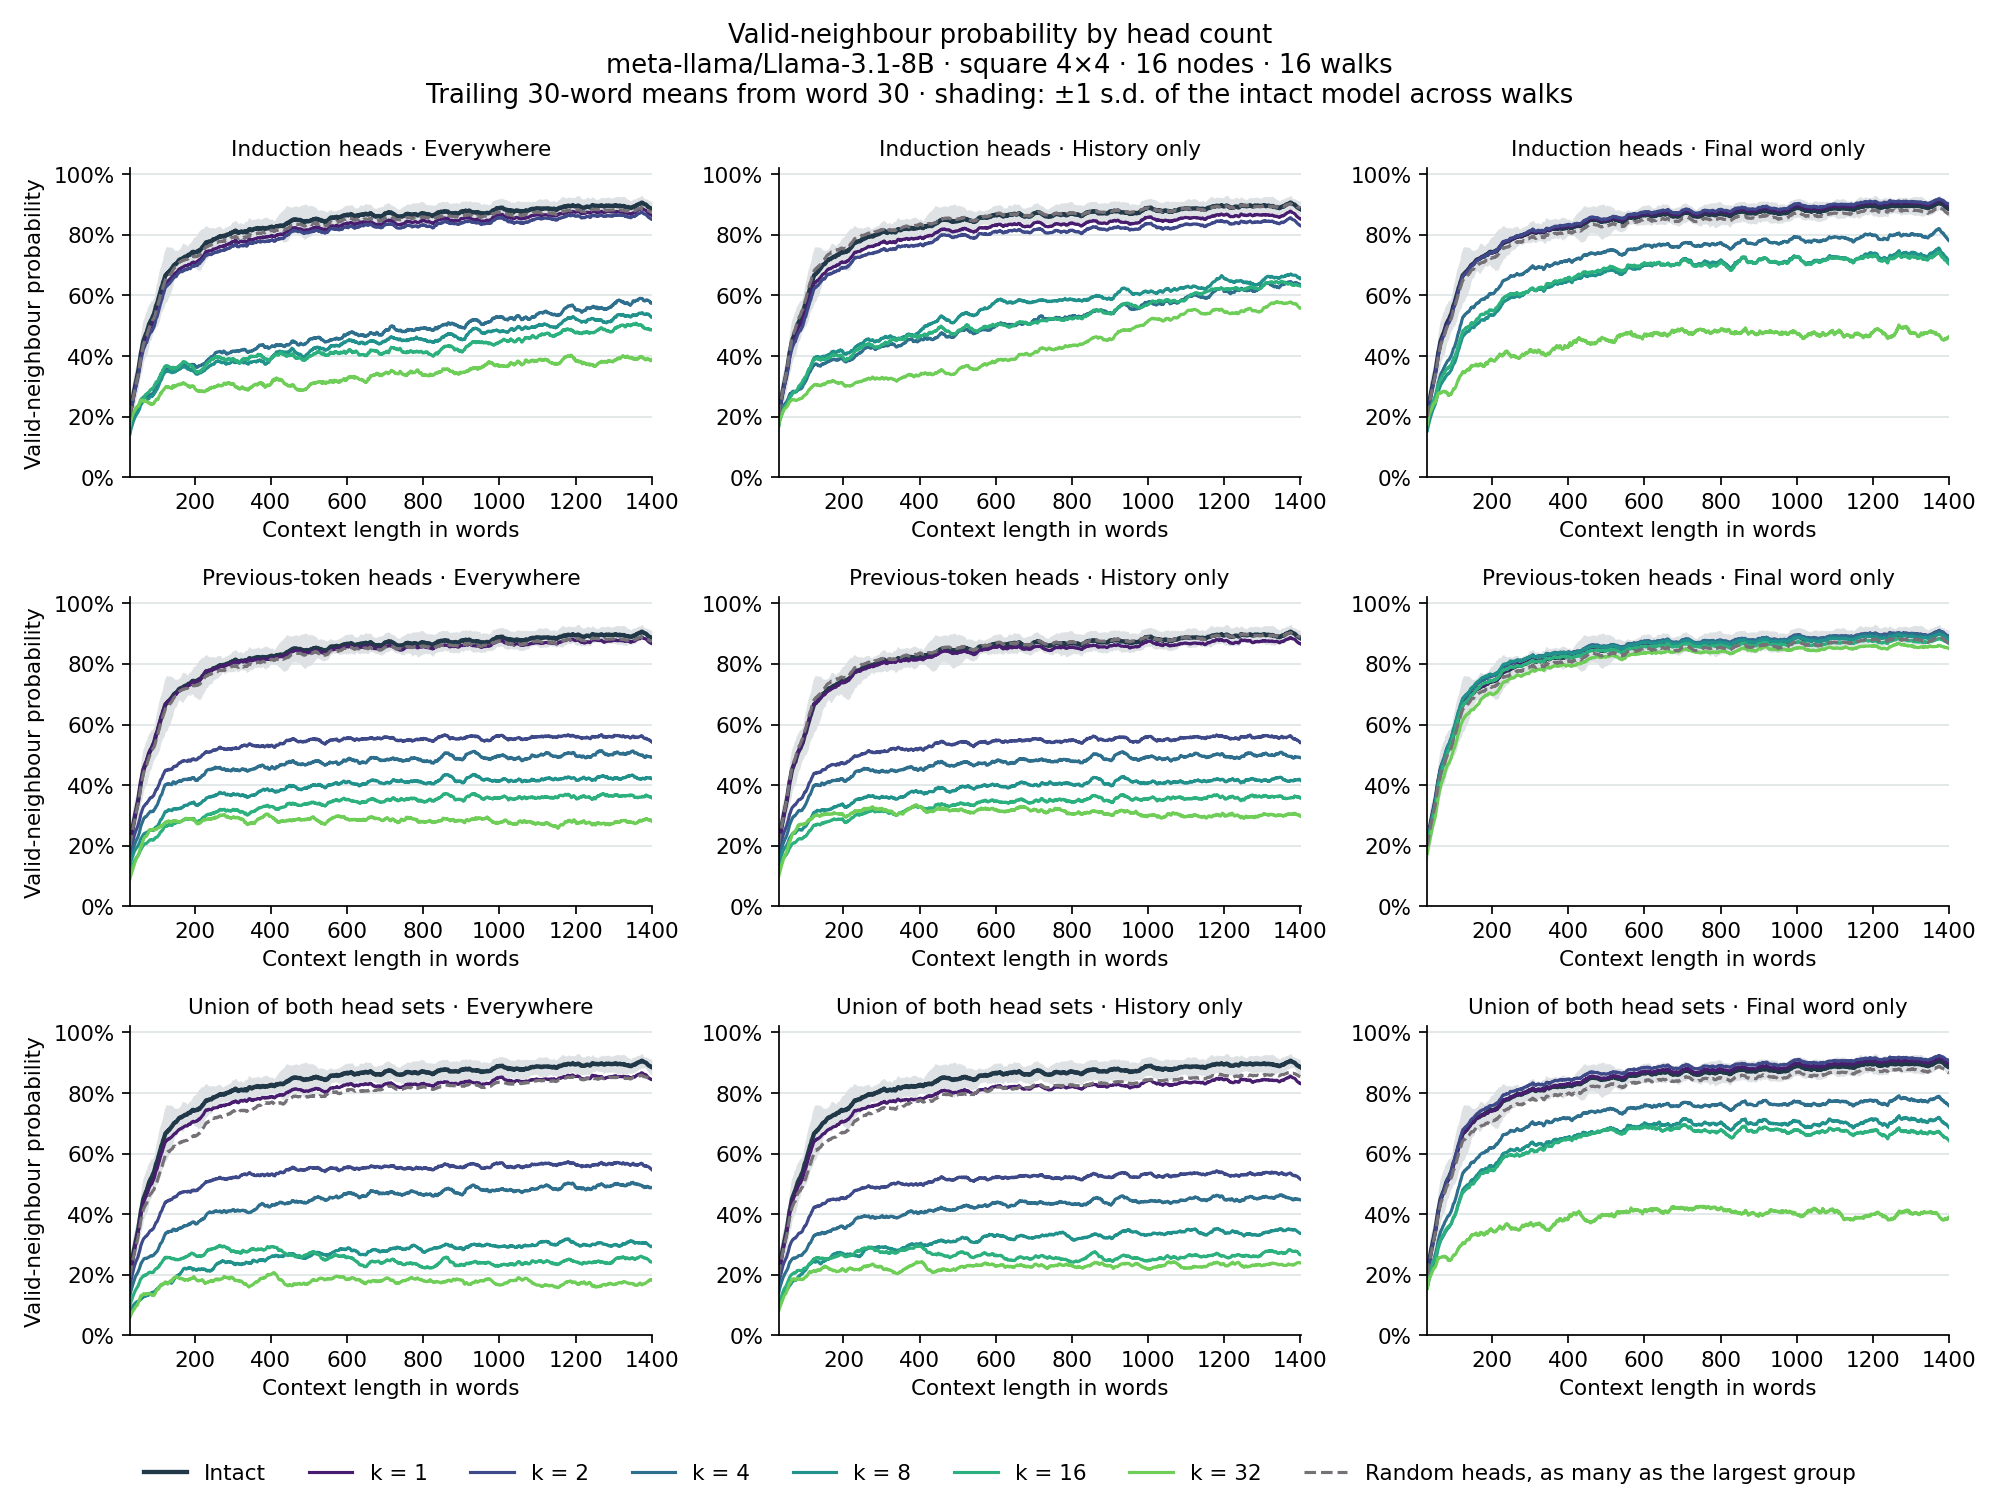
\includegraphics[width=0.92\textwidth]{accuracy-by-head-count.png}
  \caption{Valid-neighbour probability (the rule-following accuracy of \citet{park2025}) against context length, for
  Llama-3.1-8B on the $4\times 4$ grid with Park et al.'s words (16 walks of 1,400 words). The top-$k$ heads of each
  group are ablated everywhere, only in the history, or only at the final token (columns). Rows: induction heads,
  previous-token heads and their union. Dashed grey line: random heads, as many as the largest group (mean of four
  draws).}
  \label{fig:headcount}
\end{figure}

\begin{figure}[p]
  \centering
  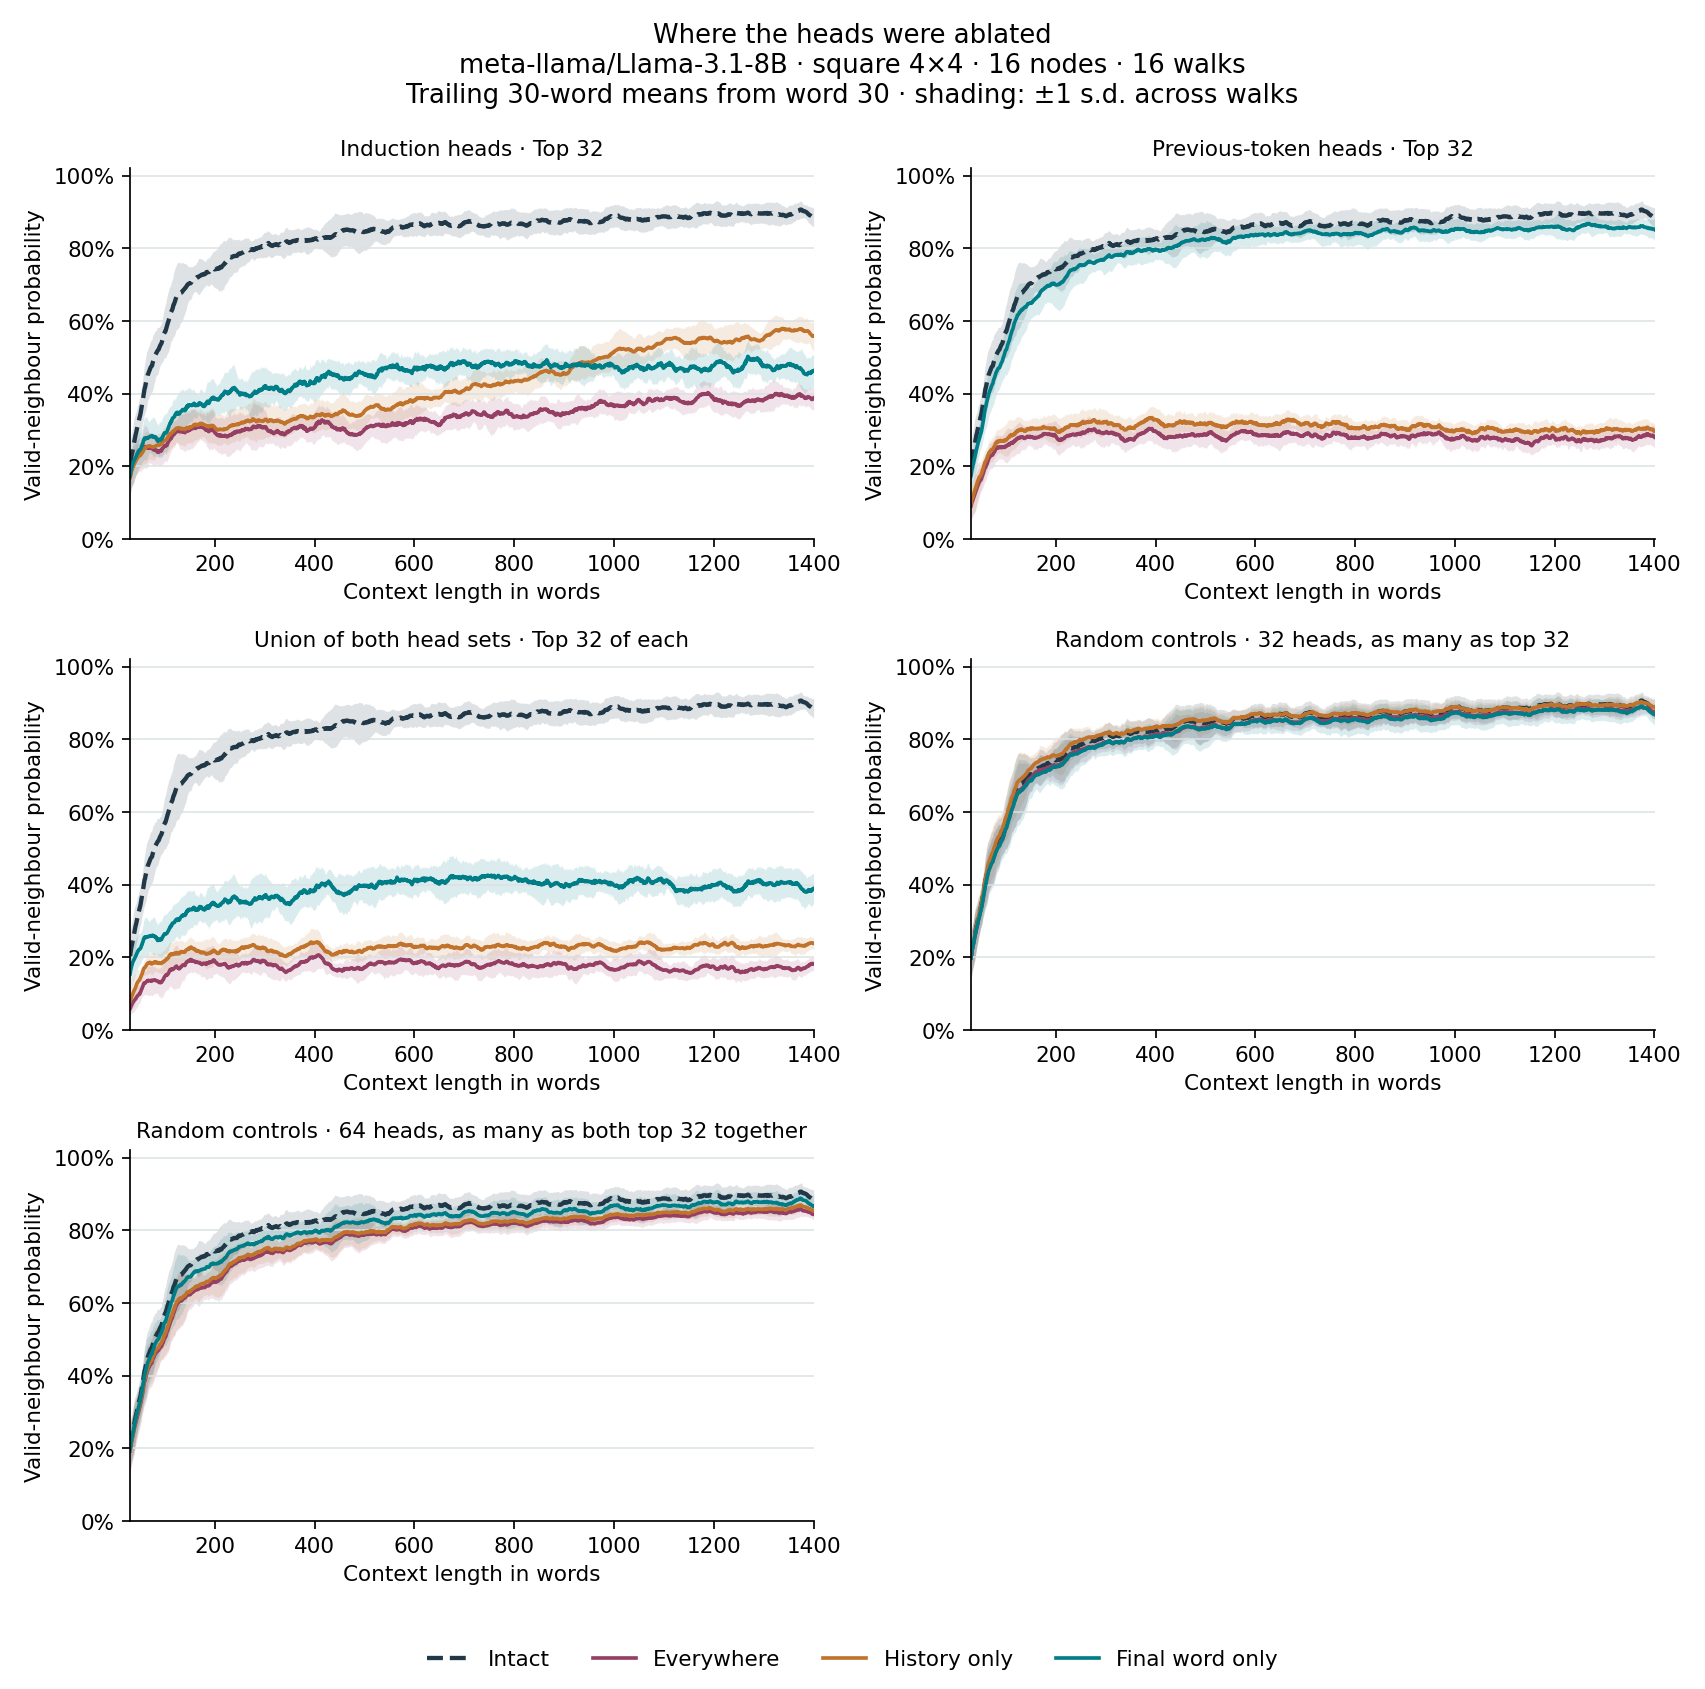
\includegraphics[width=0.9\textwidth]{accuracy-by-scope.png}
  \caption{Same run as Figure~\ref{fig:headcount}, with the three ablation scopes in one panel for each group of 32
  heads (64 for the union) and for the random controls of the same sizes.}
  \label{fig:scope}
\end{figure}

\begin{figure}[tbp]
  \centering
  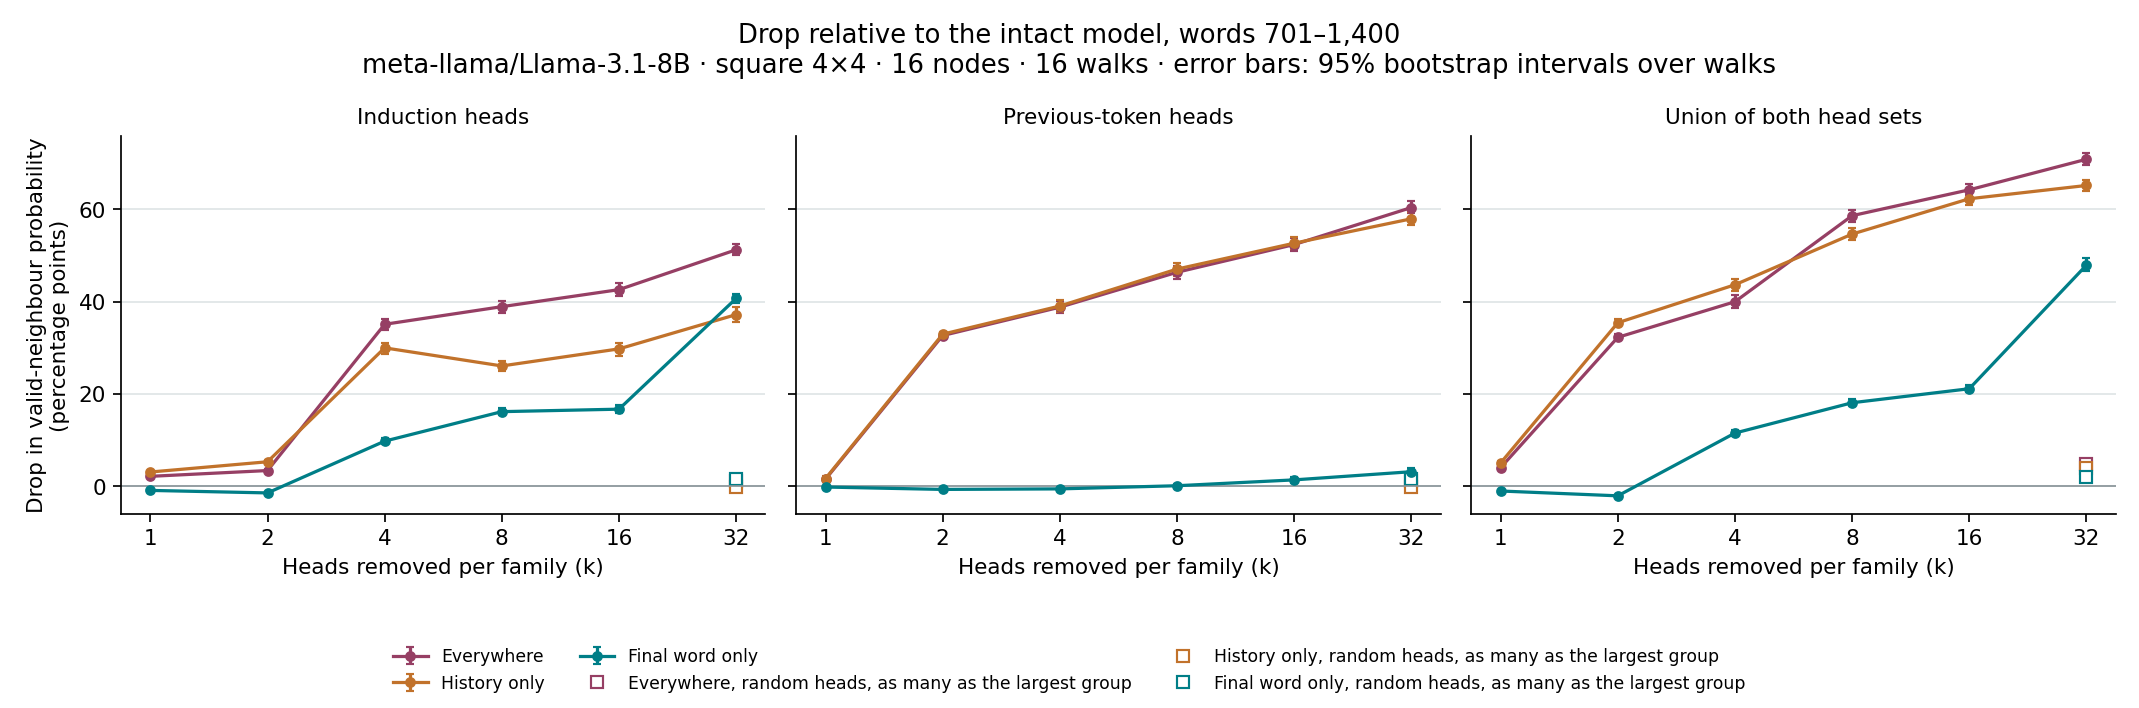
\includegraphics[width=\textwidth]{effects-by-head-count.png}
  \caption{Drop in valid-neighbour probability relative to the intact model over words 701--1,400, against the number
  of heads ablated per type ($k$), for each scope. Squares: random controls (mean of four draws). Error bars: 95\%
  bootstrap intervals over walks.}
  \label{fig:effects}
\end{figure}

\begin{figure}[tbp]
  \centering
  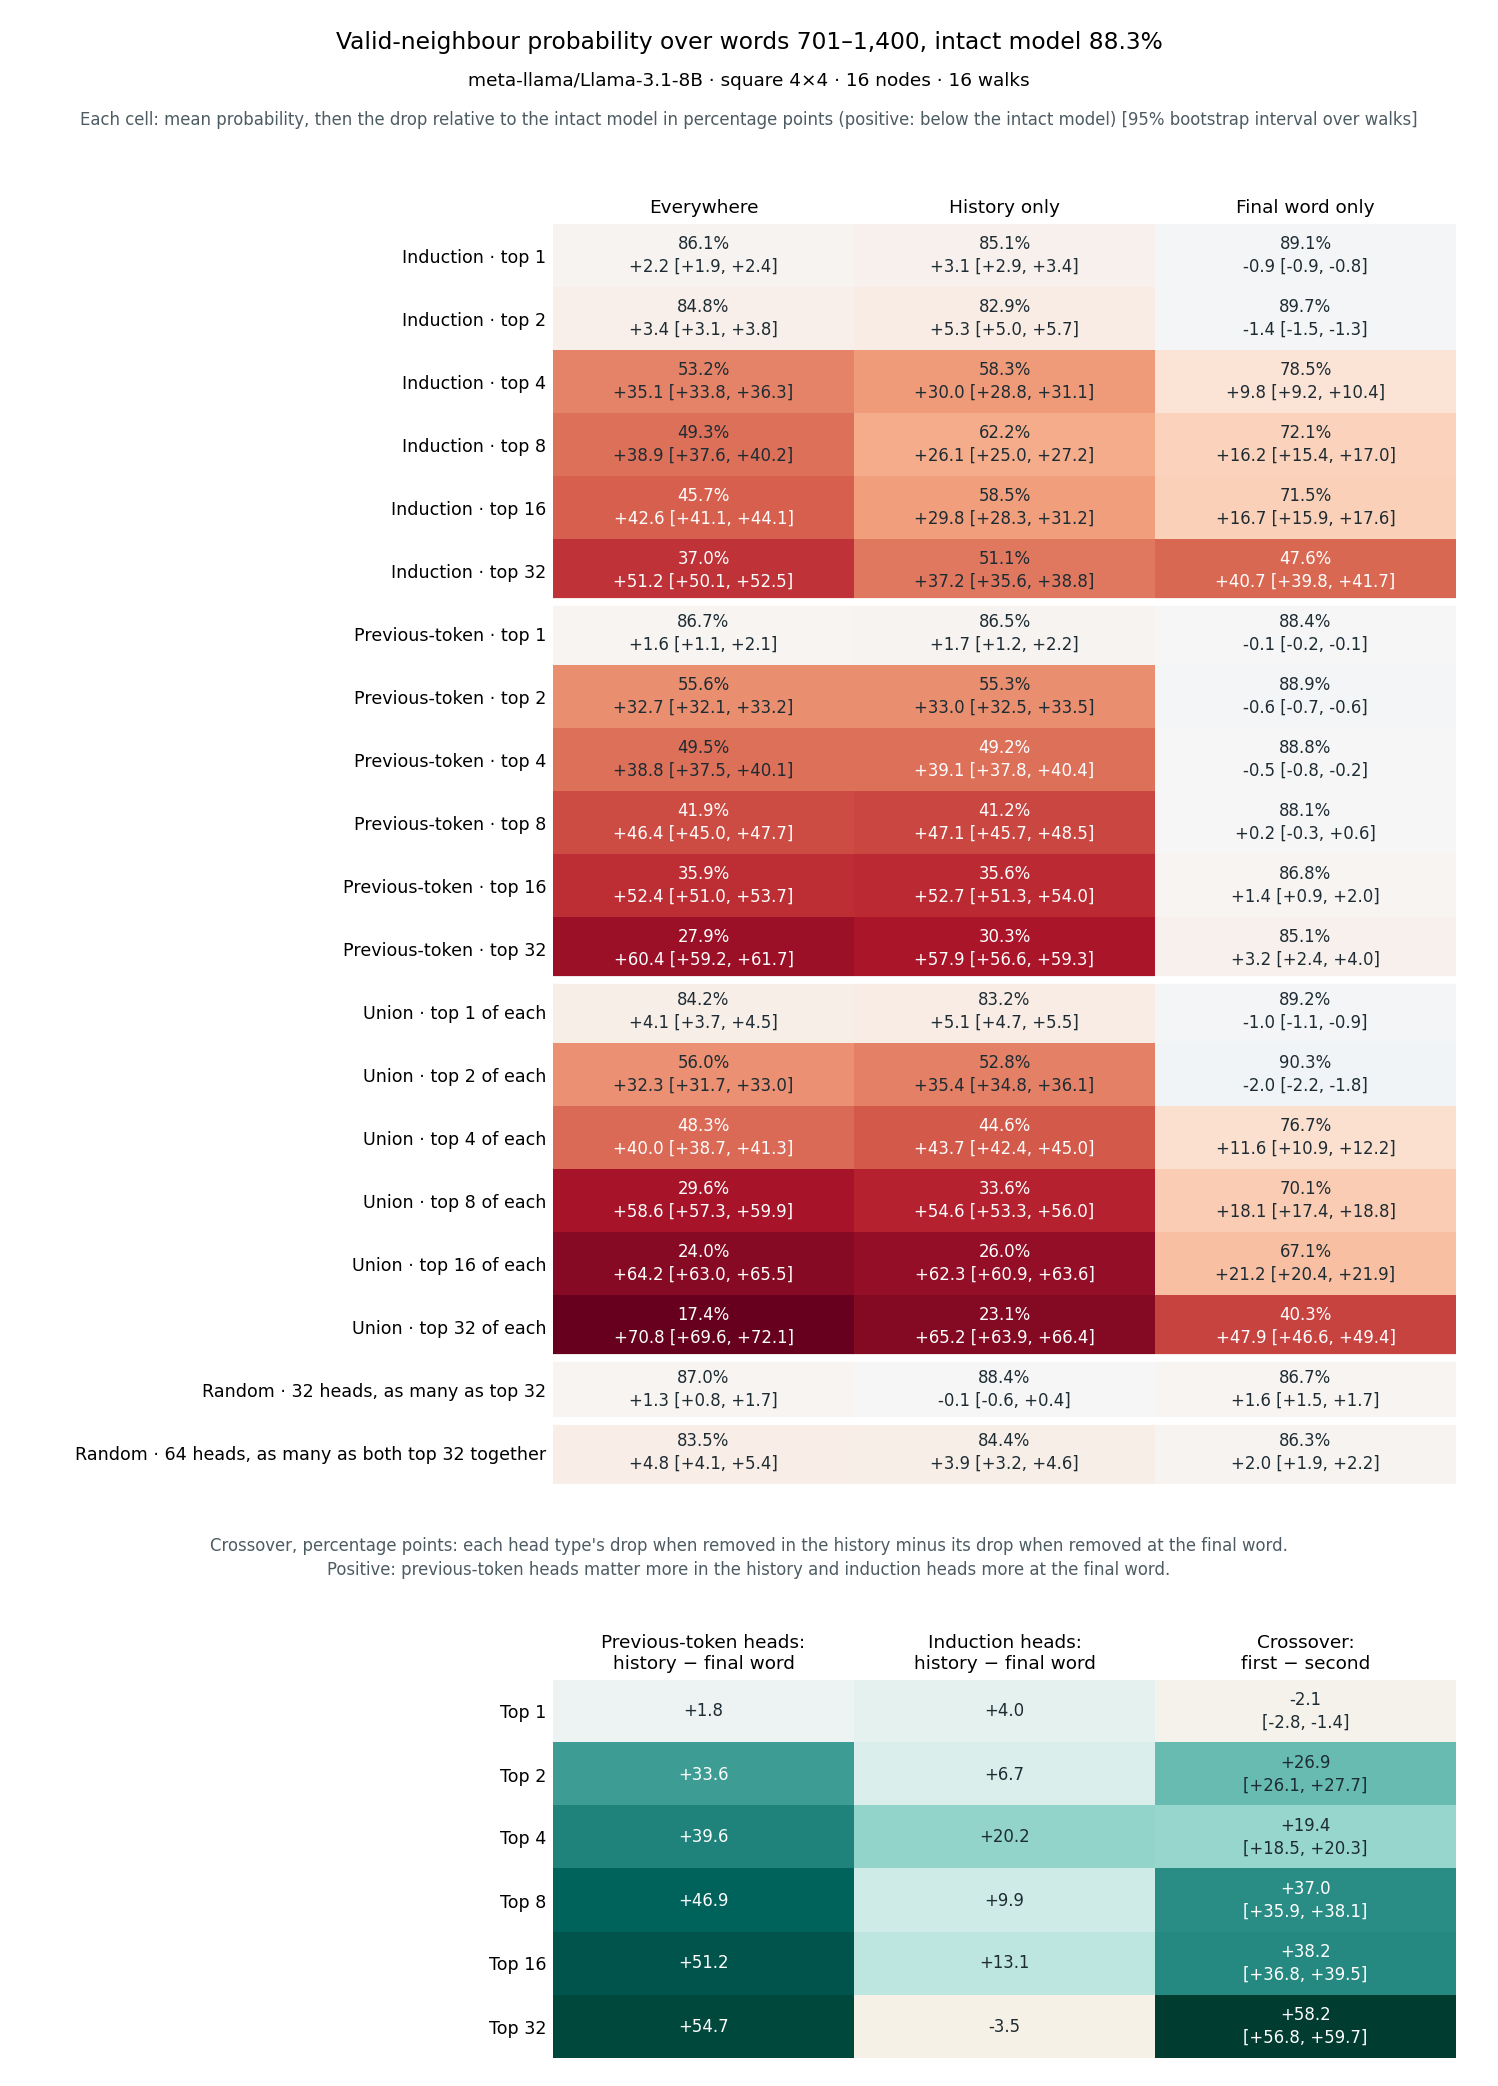
\includegraphics[width=0.8\textwidth]{effects-table.png}
  \caption{The numbers behind Figure~\ref{fig:effects}: mean valid-neighbour probability over words 701--1,400 and
  its drop relative to the intact model (88.3\%), in percentage points, with 95\% bootstrap intervals over walks.
  Bottom: for each $k$, the drop of each head type when ablated in the history minus its drop when ablated at the
  final token, and the difference of the two (the \emph{crossover}), which is positive when previous-token heads
  matter more in the history and induction heads more at the final token.}
  \label{fig:table}
\end{figure}

\begin{table}[tbp]
  \centering
  \small
  \caption{Drops in valid-neighbour probability for $k = 32$ (percentage points, words 701--1,400, 16 walks), with
  95\% bootstrap intervals over walks, from an additional run with the same walks, which reproduces the drops of
  Figure~\ref{fig:table}. For each group, the second line gives the drop beyond a layer-matched control (as many random
  heads from the same layers, averaged over four draws); the last three rows give the controls themselves.}
  \label{tab:k32}
  \begin{tabular}{lccc}
    \toprule
    & Everywhere & History only & Final token only \\
    \midrule
    Induction, top 32 & 51.2 [50.1, 52.5] & 37.2 [35.6, 38.8] & 40.7 [39.8, 41.7] \\
    \quad beyond the control & 51.1 [50.3, 52.1] & 39.5 [38.3, 40.7] & 38.2 [37.2, 39.2] \\
    Previous-token, top 32 & 60.4 [59.2, 61.7] & 57.9 [56.6, 59.3] & 3.2 [2.4, 4.0] \\
    \quad beyond the control & 51.7 [50.7, 52.8] & 50.7 [49.7, 51.7] & 2.4 [1.5, 3.3] \\
    Union, top 32 of each & 70.8 [69.6, 72.1] & 65.2 [63.9, 66.4] & 47.9 [46.6, 49.4] \\
    \quad beyond the control & 55.6 [54.6, 56.7] & 54.7 [53.7, 55.7] & 44.1 [42.6, 45.7] \\
    \midrule
    Layer-matched control: induction & 0.1 [$-$0.3, 0.5] & $-$2.3 [$-$2.8, $-$1.7] & 2.5 [2.3, 2.7] \\
    \quad previous-token & 8.7 [7.9, 9.5] & 7.3 [6.5, 8.0] & 0.8 [0.7, 0.9] \\
    \quad union & 15.2 [14.4, 16.0] & 10.5 [9.7, 11.2] & 3.8 [3.6, 4.0] \\
    \bottomrule
  \end{tabular}
\end{table}

Interestingly, ablating the top two induction heads has a negligible effect on accuracy, while ablating more of them
can have a much larger effect (here, at most 5 percentage points for the top 2, against 35 for the top 4 when ablated
everywhere). This suggests that several top induction heads might contribute to the accuracy through
an OR-like mechanism, which works just as well when some of the heads are missing; alternatively, the third and fourth
heads of the ranking may simply matter more for this task than the first two, which ablating heads individually would
distinguish.

We also show how the internal representations change with the ablations, by projecting the activations at a late
layer (the residual stream entering block 26 for Llama-3.1-8B), averaged for each word over the last 200 words of each
walk, onto their first two principal components (Figure~\ref{fig:pca}). In the final-token and history conditions,
every word of this window is treated as the final token of its own prefix: its hidden state is computed with the heads
removed only at that word (final token only) or only at the earlier positions (history only). Each panel reports the
\emph{overlap} between the plane of the first two principal components and the plane of the two smoothest non-constant
eigenvectors of the graph Laplacian (1 means the same plane). On the grid of \citet{park2025}, we replicate the finding
of \citet{arditi2026} that ablating previous-token heads disrupts the geometry (overlap 0.39, against 0.97 for the intact model), while ablating induction heads leaves it
largely intact (0.95). The layer-matched controls leave it intact in all three conditions (0.94 to 0.97), so the
disruption is specific to the previous-token heads. We also find that ablating
previous-token heads only at the word itself already degrades the geometry (0.72), suggesting that previous-token
mixing has a substantial effect on the geometric representation, as \citet{arditi2026} argued with a toy-model
experiment; ablating them only in the history degrades it even more (0.63). Interestingly, ablating induction heads
only at the word itself also changes the geometry (0.82), more than ablating them everywhere (0.95), suggesting that
information about the words that followed each word earlier in the walk is used in the representation of that word.

\begin{figure}[tbp]
  \centering
  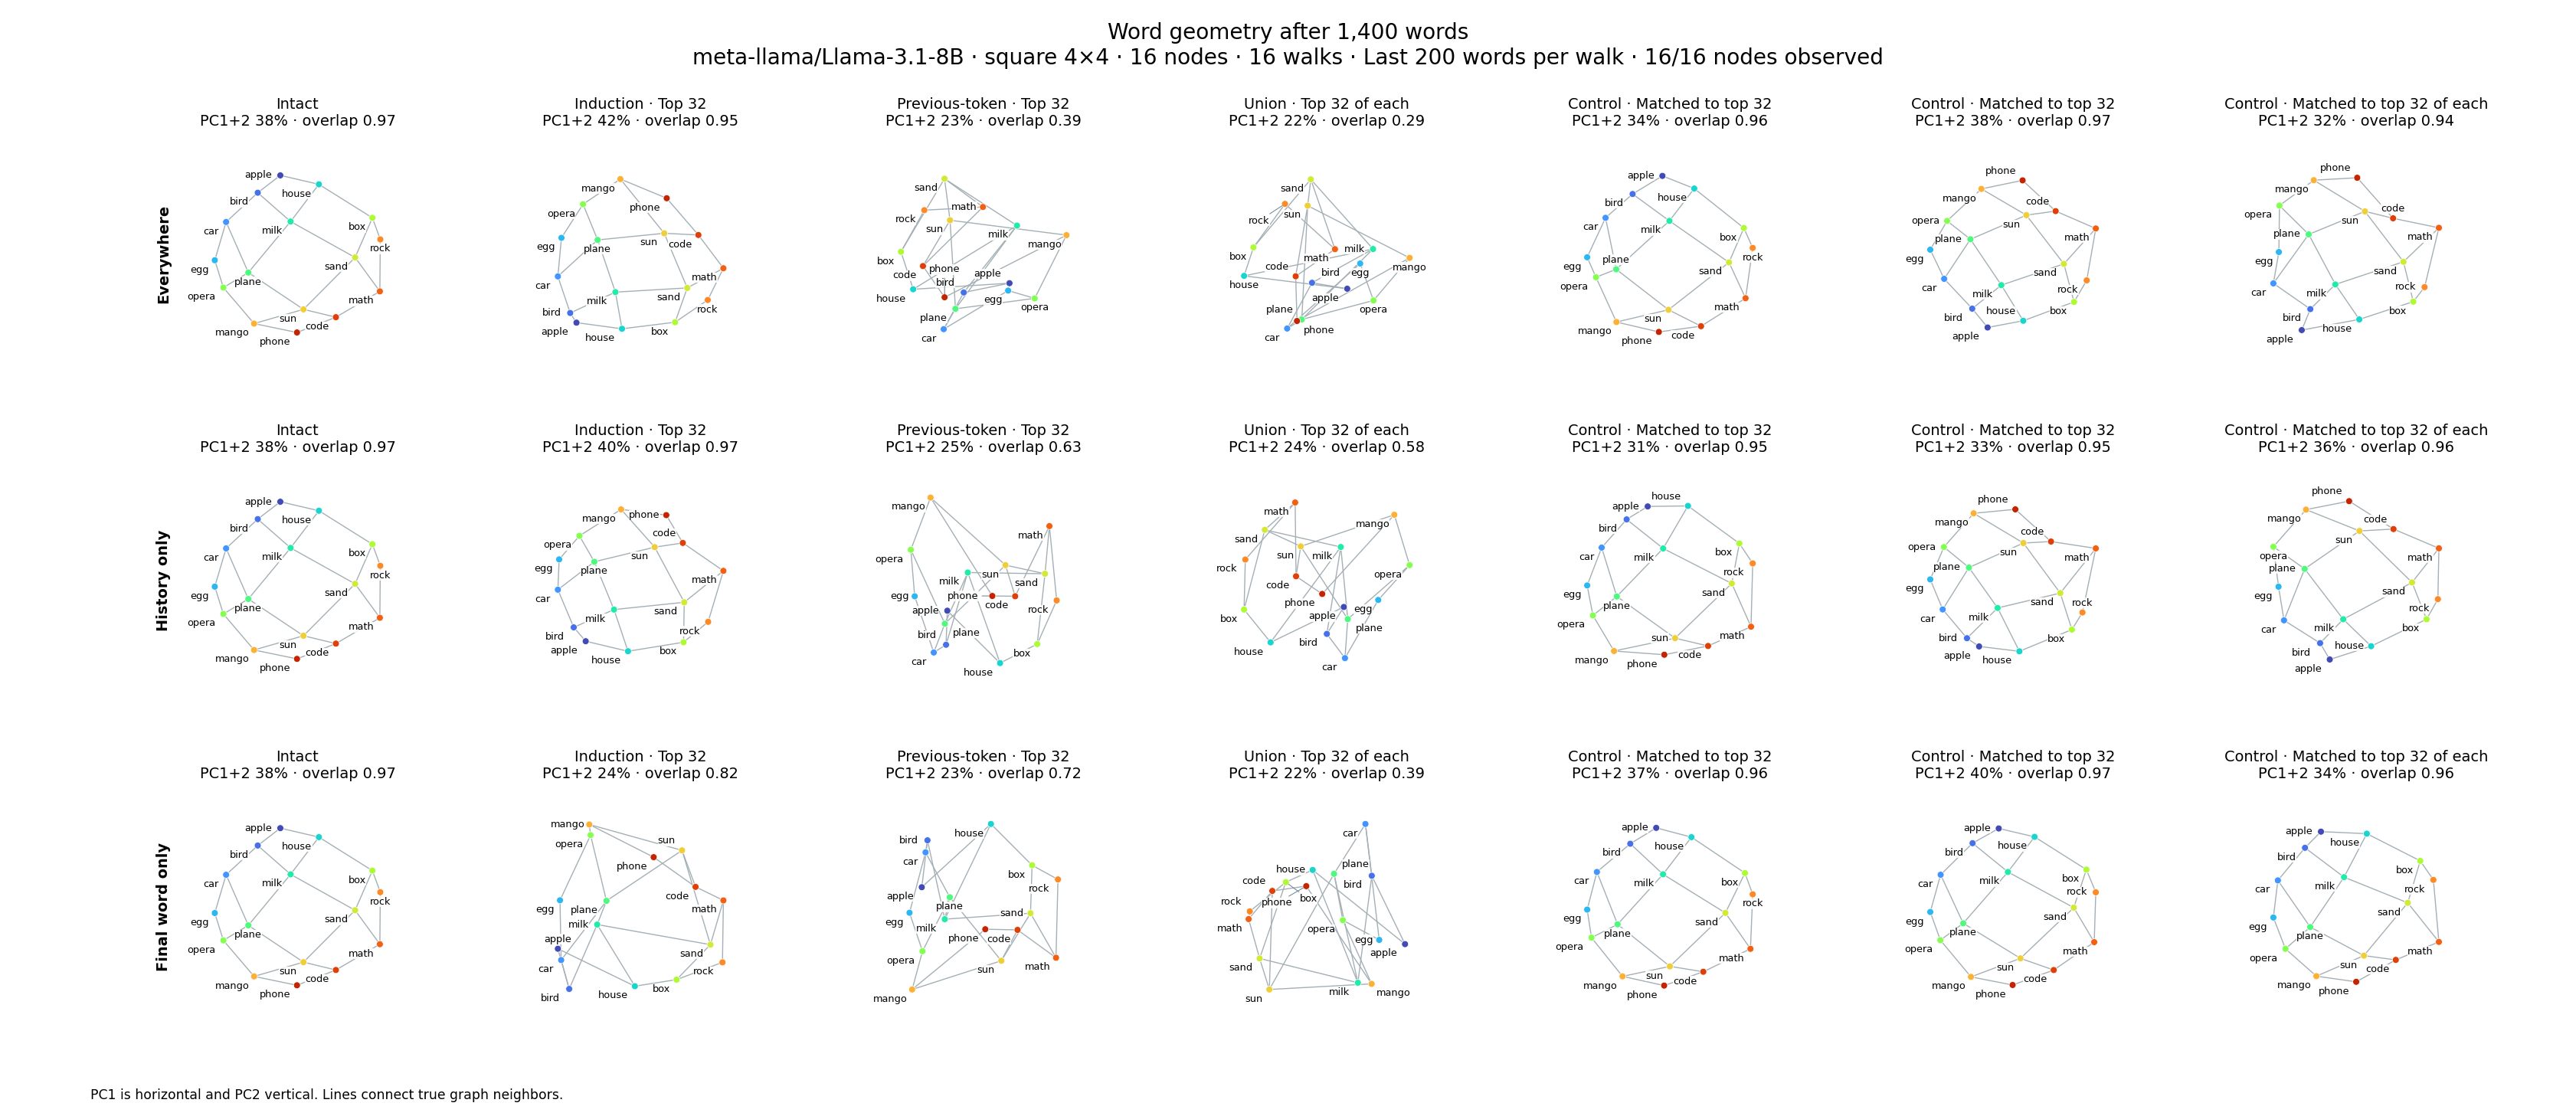
\includegraphics[width=\textwidth]{pca-final-window.png}
  \caption{Projection onto the first two principal components of each word's mean hidden state entering block 26
  (last 200 words of each walk), for the additional run of Table~\ref{tab:k32}, which uses the same walks as
  Figure~\ref{fig:headcount} and gives the same maps for the identified heads. Rows: ablation scope; columns: intact
  model, top-32 induction and previous-token heads, their union, and the three layer-matched controls (first draw).
  Lines join neighbours in the graph.}
  \label{fig:pca}
\end{figure}

The effect on the geometry can depend strongly on the words, as Figure~\ref{fig:pca-seeds} shows for words drawn at
random with seeds 42, 44 and 46 (again with 16 walks of 1,400 words). With seed 44, the grid appears in the intact model
and the ablations behave as with Park et al.'s words: removing previous-token heads everywhere disrupts the geometry
(overlap 0.34), while removing induction heads leaves it intact (0.95). Here, however, unlike with Park et al.'s words,
the layer-matched control of the previous-token heads also degrades it (0.59), so part of this effect may come from removing heads in those layers
rather than from the previous-token heads themselves. With seeds 42 and 46, the grid does not appear even in the intact
model (overlap 0.47 and 0.60), because the bipartite structure of the graph prevails. This suggests that the graph
geometry does not always arise, at least in the first two principal components; we may investigate this further in
future experiments. Interestingly, the grid geometry can be recovered when some heads are ablated, for example all
top-32 induction heads (overlap 0.96 and 0.93), but also 64 random heads (0.96 and 0.88), so this recovery is not
specific to the heads of the circuit, although most layer-matched controls leave the bipartite structure in place.

\begin{figure}[tbp]
  \centering
  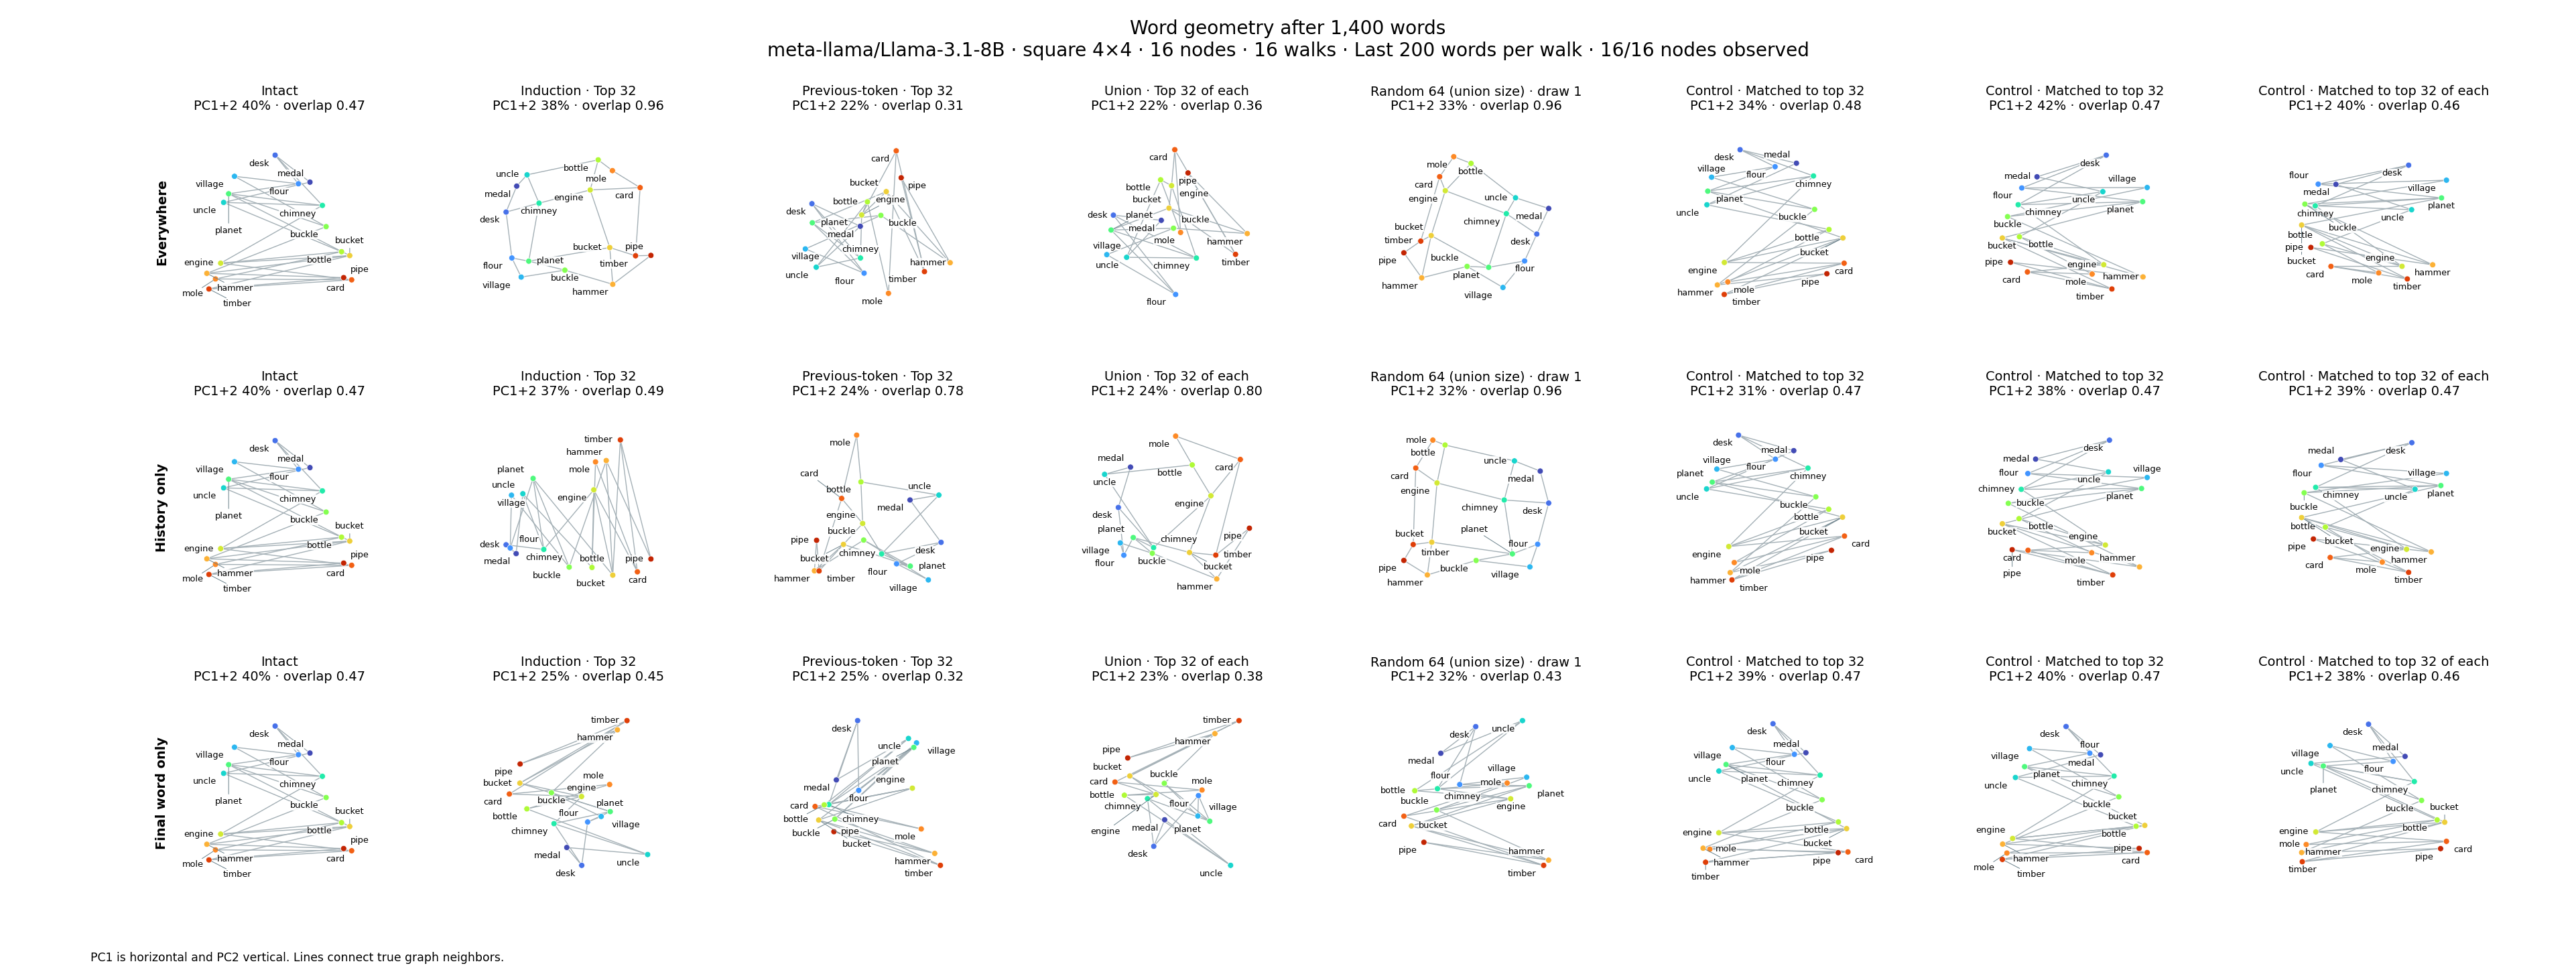
\includegraphics[width=\textwidth]{pca-final-window-42.png}\\[2pt]
  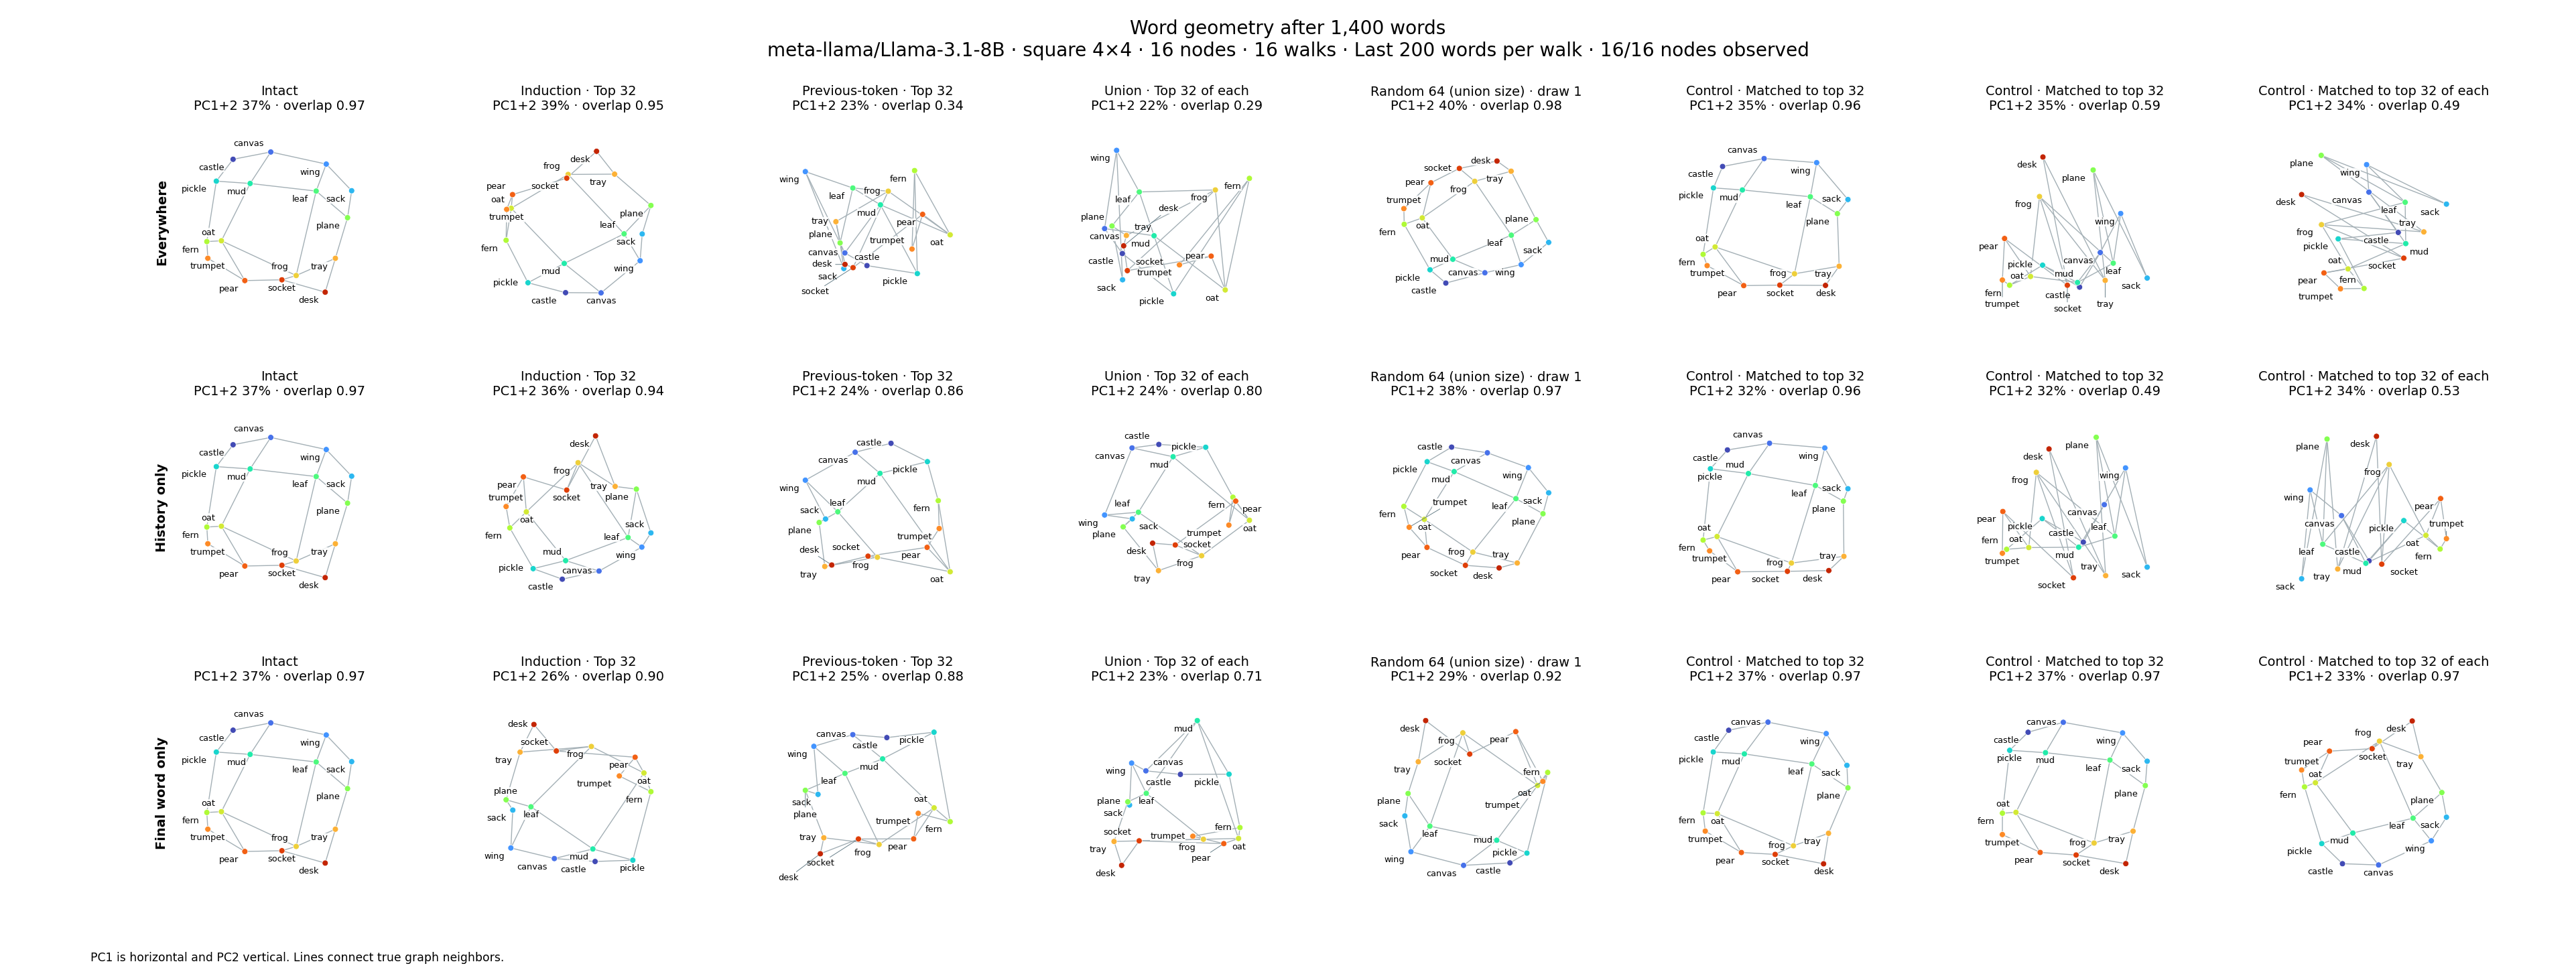
\includegraphics[width=\textwidth]{pca-final-window-44.png}\\[2pt]
  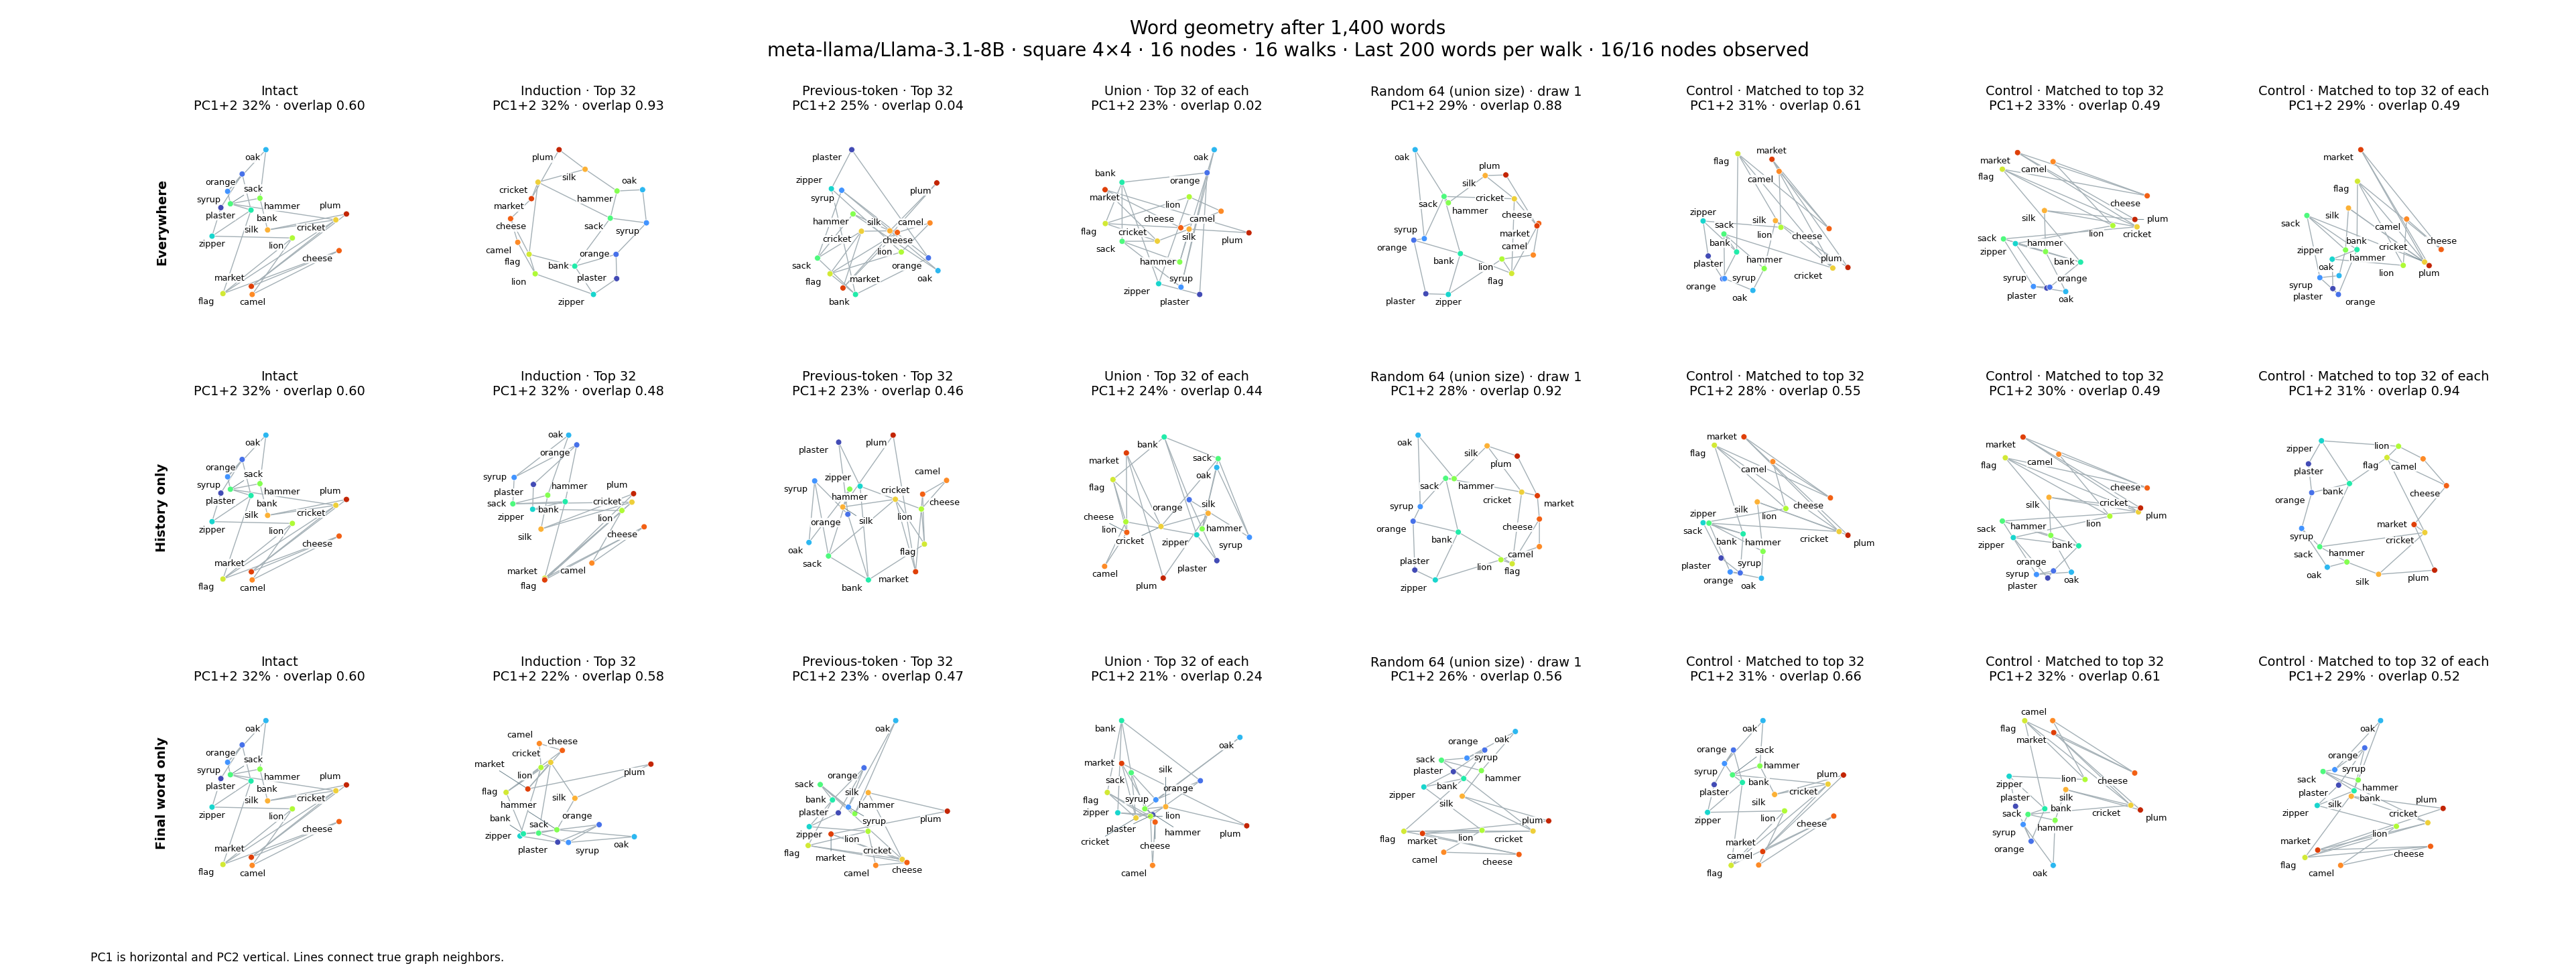
\includegraphics[width=\textwidth]{pca-final-window-46.png}
  \caption{As Figure~\ref{fig:pca}, for words drawn at random with seed 42 (top), 44 (middle) and 46 (bottom), with one
  more column for 64 random heads (first draw).}
  \label{fig:pca-seeds}
\end{figure}

\section{Experiment 2: accuracy curve fitting and scaling}

In our second experiment, we fit the accuracy curve of in-context graph learning with the descriptions proposed by
\citet{park2025} and by \citet{kowalyshyn2026}.

\citet{park2025} describe the curve with a piecewise-linear fit in log(context length): the accuracy first stagnates,
as the model has not yet learned the graph structure, then rises more steeply until it approaches its final ceiling.
They also analyse where in the context the slope changes for different graph topologies and sizes, and suggest that
this transition point might scale as a power law in the graph size (with parameters that depend on the topology).

\citet{kowalyshyn2026}, in an experiment in which the model reads random walks on two different graphs one after the
other, propose a Bayesian belief model in which the accuracy of the predictions for the current walk rises as
\[
  \hat{p}(N) = p_0 + (q - p_0)\,\sigma\!\left(b + \gamma N^{1-\alpha}\right),
\]
where $\sigma$ is the logistic function, $N$ the context length, $p_0$ the initial accuracy before learning starts, $q$
the final ceiling accuracy, $b$ an initial bias towards or against the particular graph hypothesis, $\gamma$ the rate
at which new observations influence the model, and $\alpha$ the rate of diminishing returns from prolonged observation
of the same walk. The midpoint of the rise, where the accuracy is halfway between $p_0$ and $q$, is
$N^* = (-b/\gamma)^{1/(1-\alpha)}$.

We compare our accuracy curves with both models. For the piecewise-linear fit, we fit two lines to the accuracy as a
function of $\log N$, requiring the second to be steeper than the first (we are looking for where learning begins),
and optionally a third, flatter line for the plateau. We call $t_c$ the point at which learning begins. For the belief
curve, we fit all the parameters: \citet{kowalyshyn2026} estimate $p_0$ from the first 100 tokens, but we fit it
because for small graphs the accuracy starts rising earlier. Since the fit is unreliable when the walk is too short to
approach the plateau, the notebook accepts a fit as reliable only if, by the end of the walk, the accuracy has covered
at least 93\% of the rise from $p_0$ to $q$, no fitted parameter lies at the edge of its search range (except $p_0$,
which may be zero), and $N^*$ falls within the context window. Moreover, since the curve is an average over walks, and
averaging walks that each jump at different times could by itself produce a sigmoid-like curve, the notebook also
checks the shape of the single walks.

In our experiments, the belief-curve model of \citet{kowalyshyn2026} usually describes the accuracy curves better than
the two lines, both by held-out error (fitting on half of the walks and testing on the other half) and by BIC. In a few cases its fit is not reliable, often because the initial bias $b$ is pushed to the
negative end of its range; this happens mostly for large ring graphs.

Figure~\ref{fig:fits} shows the results for Llama-3.1-8B on the $4\times 4$ grid of \citet{park2025}, with 32 walks of
4,000 tokens; other results are in the repository together with the notebooks. The top panel shows the accuracy (each
point is the mean over walks and over a bin of context lengths, the bins being equally spaced on a log axis) together
with the two fits, and the \emph{revealed share}, a measure of how much of the local graph structure the walk has
shown: the fraction of the current word's neighbours that have already appeared immediately after it earlier in the
walk. The middle and bottom panels show the normalized Dirichlet energy of the activations (computed as in
\citet{kowalyshyn2026}) and the $R^2$ of the PCA projection against the true drawing of the graph (one minus the
Procrustes disparity), each with a baseline in which the words are placed at random. Figure~\ref{fig:pca-pictures}
shows the PCA projections at context lengths close to $N^*/4$, $N^*$, $4N^*$ and at the end of the walk.

In this run, the belief curve has the lower held-out error in all 20 random splits of the walks (RMS 0.032 against
0.035), and BIC favours it by 10.8. Its midpoint is $N^* = 64$ tokens (68\% bootstrap interval 50--74), while the two
lines meet at $t_c = 33$. The single walks have the S-shape themselves: the rise of a single walk is on median 0.87
times as wide as that of the averaged curve, and the midpoints of the walks spread over only 0.15 decades, much closer
to simulated smooth walks (1.12 and 0) than to simulated walks that each jump abruptly (0.03 and 0.63). On single walks,
which are noisier, the two descriptions are closer: the belief curve has the lower held-out error in 78\% of the walks,
but the lower BIC in only 38\%.

\begin{figure}[tbp]
  \centering
  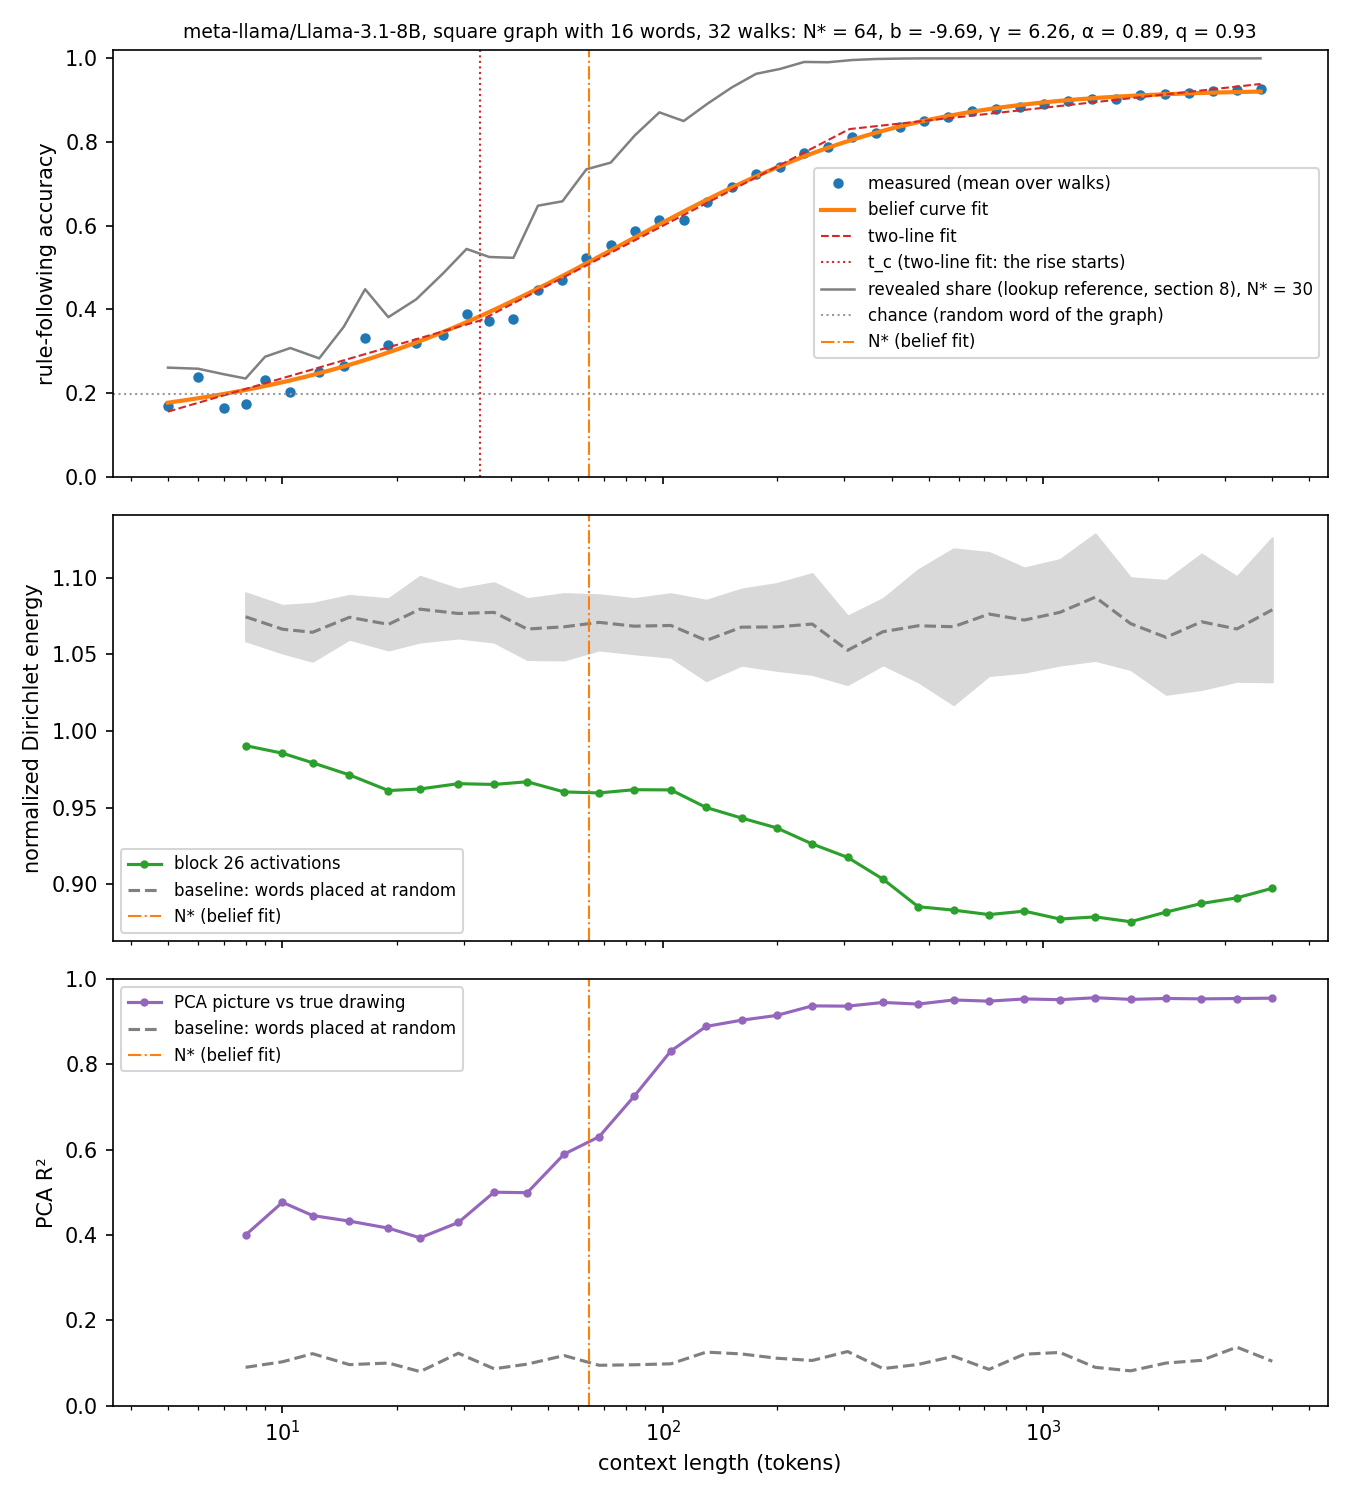
\includegraphics[width=0.78\textwidth]{accuracy_energy_r2.png}
  \caption{Llama-3.1-8B on the $4\times 4$ grid with Park et al.'s words (32 walks of 4,000 tokens). Top: accuracy
  with the belief-curve and two-line fits, and the revealed share (grey). Middle: normalized Dirichlet energy of the
  block-26 activations. Bottom: $R^2$ of the PCA projection against the true drawing. Grey dashed lines: words placed
  at random. Vertical lines: $N^*$ (belief fit) and $t_c$ (two-line fit).}
  \label{fig:fits}
\end{figure}

\begin{figure}[tbp]
  \centering
  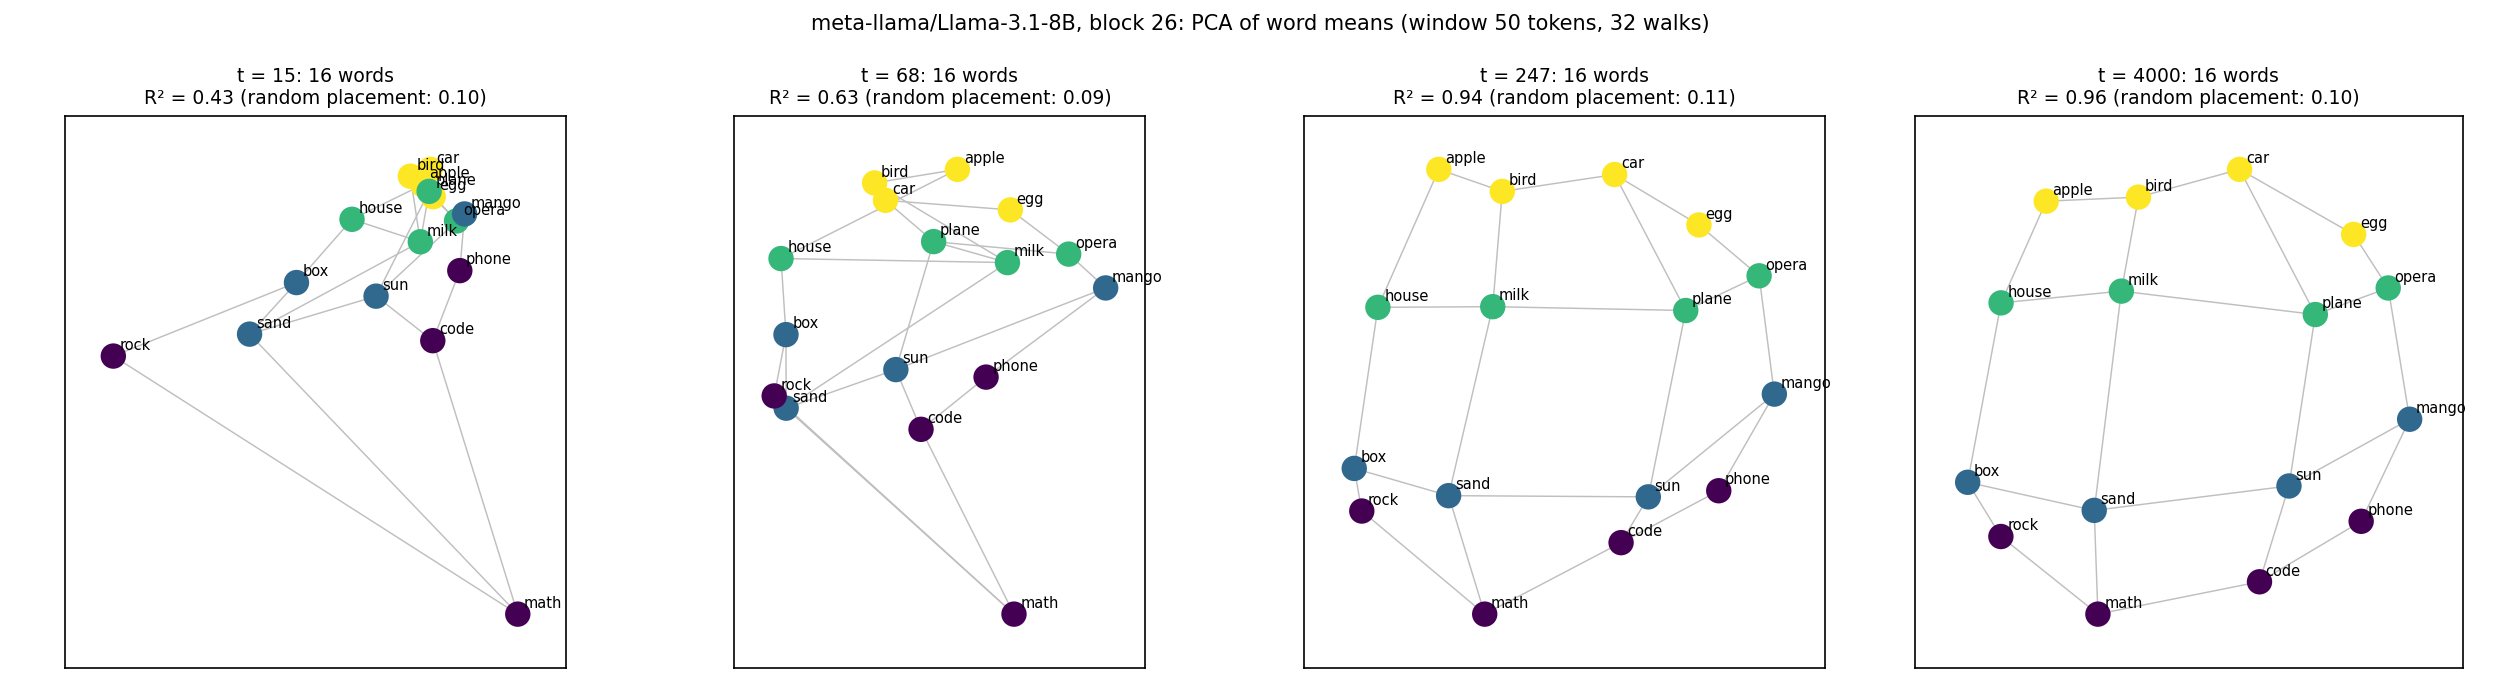
\includegraphics[width=\textwidth]{pca_pictures.png}
  \caption{PCA projections of the word means (block 26, 50-token window) at context lengths 15, 68, 247 and 4,000
  tokens, close to $N^*/4$, $N^*$, $4N^*$ and the end of the walk ($N^* = 64$).}
  \label{fig:pca-pictures}
\end{figure}

Finally, Figure~\ref{fig:scan-curves} shows the accuracy curves for square grids of different sizes, from $3\times 3$
to $12\times 12$ (obtained with the size scan of the notebook, with word seeds 0 to 4), and
Figure~\ref{fig:scan-params} shows how the fitted parameters vary with the size of the graph. The midpoint $N^*$
scales approximately as a slightly sublinear power law in the number of vertices $n$, $N^* \approx 4.75\, n^{0.89}$.
The plateau accuracy $q$ decreases slowly with size, from about 0.94 to 0.87, while the other parameters show no clear
pattern. The grey squares show the midpoint of the revealed-share curve, fitted in the same way as the accuracy curve
($N^* \approx 2.22\, n^{0.95}$). The $t_c$ of the revealed share is not very informative, because that curve rises
steeply from the very beginning.

The midpoint $N^*$ of the accuracy curve thus grows almost as fast as that of the revealed-share curve (exponents 0.89
and 0.95), staying about 1.6 to 1.9 times larger according to the fitted power laws (2.1 for the $4\times 4$ grid of
Figure~\ref{fig:fits}). This suggests that the accuracy rises roughly once the walk has shown most of each word's
neighbours right after it, so that a model that remembers which words followed earlier occurrences of the current word
can use them; this is consistent with the role of induction circuits in Experiment~1.

\begin{figure}[tbp]
  \centering
  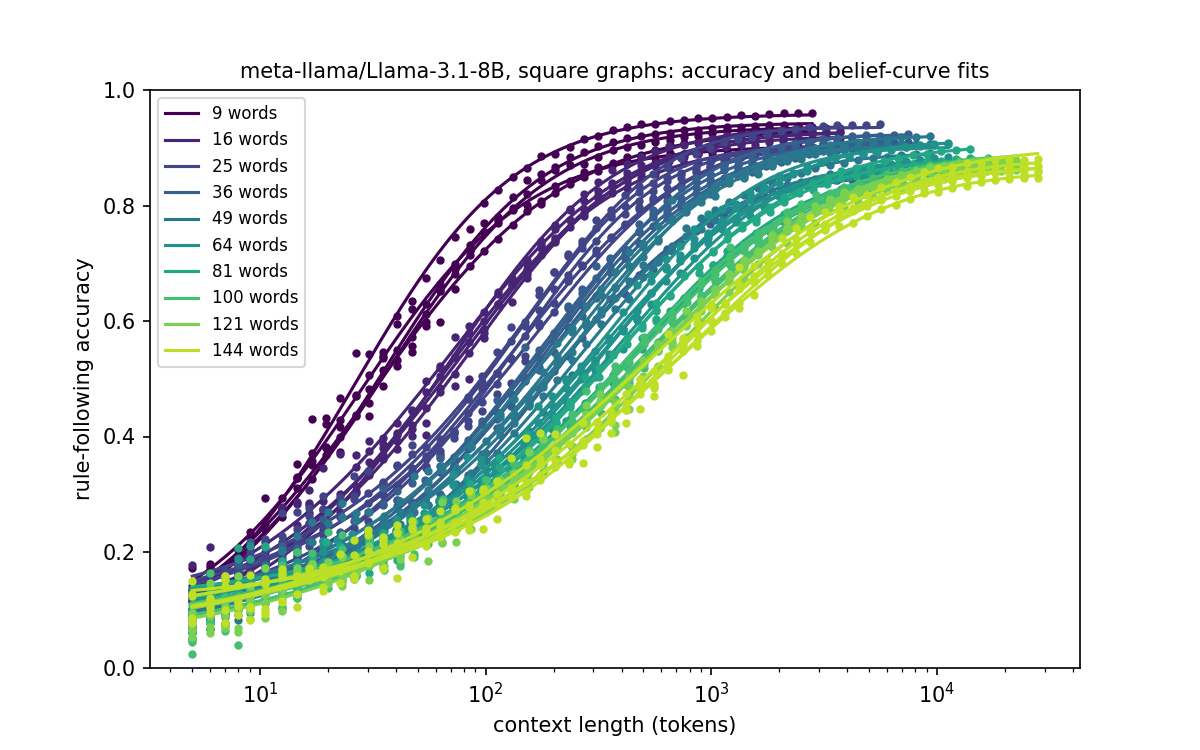
\includegraphics[width=0.8\textwidth]{scan_accuracy_curves.png}
  \caption{Accuracy and belief-curve fits for Llama-3.1-8B on square grids from $3\times 3$ to $12\times 12$ (9 to 144
  words), with five word seeds per size and 32 walks per run.}
  \label{fig:scan-curves}
\end{figure}

\begin{figure}[tbp]
  \centering
  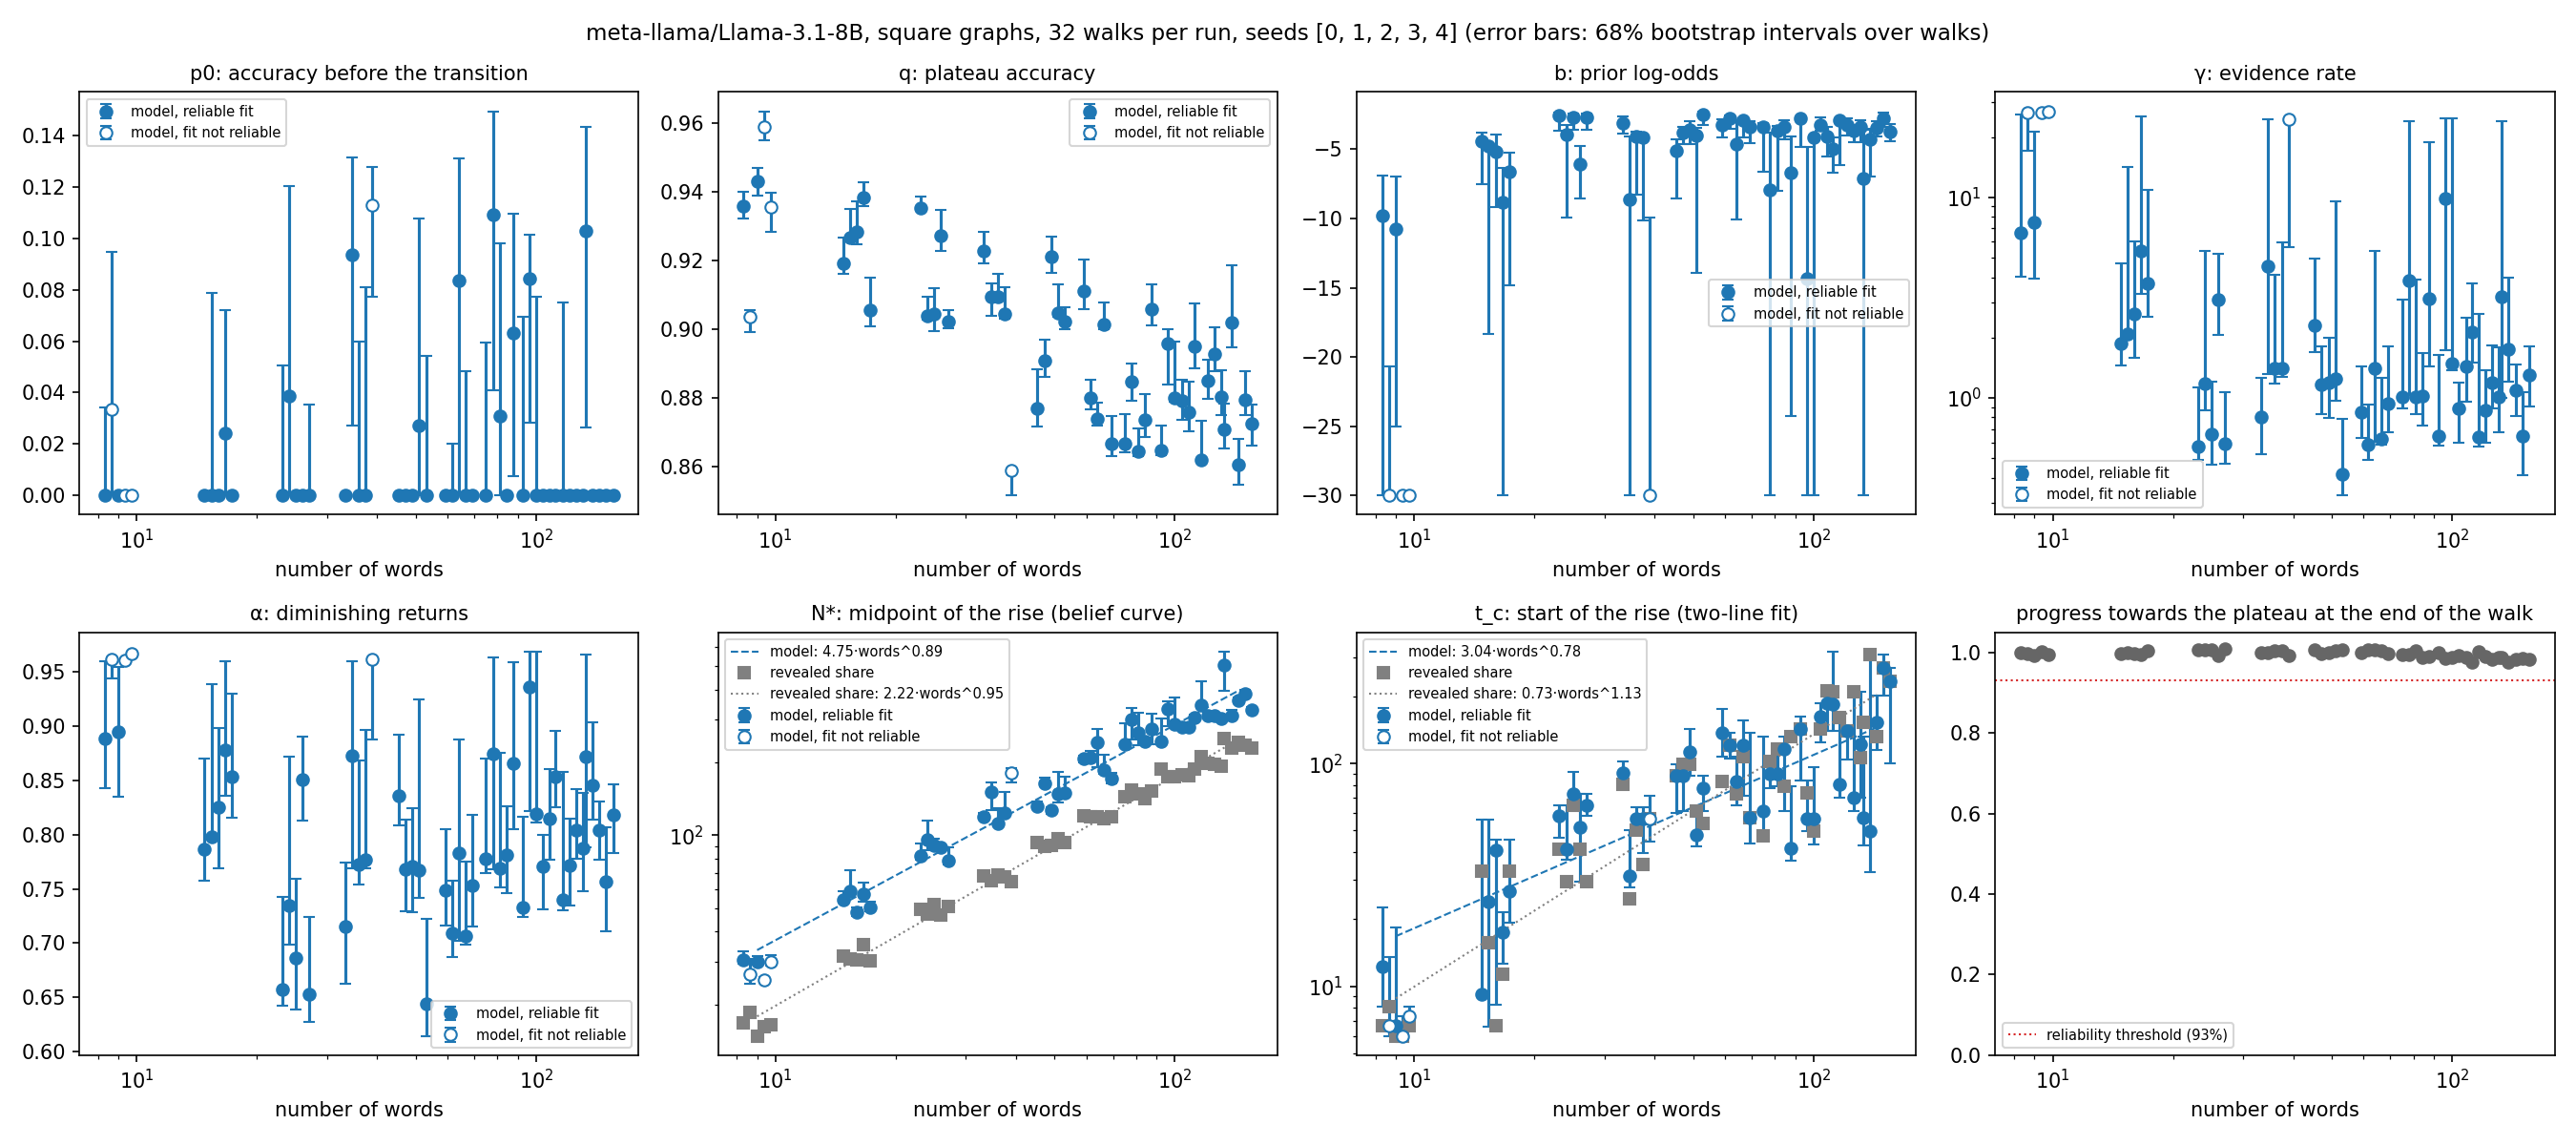
\includegraphics[width=\textwidth]{scan_parameters.png}
  \caption{Fitted parameters against the number of words, for the runs of Figure~\ref{fig:scan-curves}. Filled
  markers: reliable fits; open markers: fits that are not reliable. Grey squares: revealed share. Lines: power-law fits
  to the reliable points. Error bars: 68\% bootstrap intervals over walks.}
  \label{fig:scan-params}
\end{figure}

\section{Limitations and future work}

The results of Experiment 1 on the geometry of the representations, with and without ablations, can vary considerably
with the graph and the specific words, as the examples show. We do not
present a statistical analysis of these variations here; this may be the object of a future study. In Experiment 2,
the belief-curve fit is not always reliable, and other functions or frameworks may describe the phenomenon better.
Finally, we do not show results on world-modeling tasks like those analysed by \citet{lepori2026} and
\citet{matsutani2026}. We have run a few experiments of this kind, for example on predicting a transition of the graph
that has not yet occurred in the context but could be inferred from past moves, but we do not yet have a clear picture
to share, so we leave them to future work.

\section*{Statement on AI use}

This project was carried out with the assistance of the following AI models: Claude Opus 5.5, Claude Fable 5.2 and
GPT-6.2 Astra. The models proposed a few possible projects following the author's instructions and scanned the
relevant literature. The author chose the project, read the papers in the literature and designed the experiments
according to his own taste. The notebooks, which can be found in the repository, were generated by the AI models
following the author's instructions, then checked by the author. The author ran the notebooks on Google Colab,
interpreted the results of the experiments, and used AI to clarify some doubts and make minor improvements to the
notebooks. The text of this paper was first written by the author, then checked and polished using AI.

\begin{thebibliography}{6}

\bibitem[Arditi(2026)]{arditi2026}
A.~Arditi.
\newblock In-context learning of representations can be explained by induction circuits.
\newblock \emph{ICLR Blogposts}, 2026.
\newblock \url{https://iclr-blogposts.github.io/2026/blog/2026/iclr-induction/}.
\newblock Code and head scores: \url{https://github.com/andyrdt/iclr_induction}.

\bibitem[Kowalyshyn et~al.(2026)]{kowalyshyn2026}
K.~Kowalyshyn, T.~Duggan, D.~Little, and M.~C. Hughes.
\newblock Belief or circuitry? {C}ausal evidence for in-context graph learning.
\newblock arXiv:2605.08405, 2026.
\newblock \url{https://arxiv.org/abs/2605.08405}.

\bibitem[Lepori et~al.(2026)]{lepori2026}
M.~A. Lepori, T.~Linzen, A.~Yuan, and K.~Filippova.
\newblock Language models struggle to use representations learned in-context.
\newblock In \emph{Proceedings of the 64th Annual Meeting of the Association for Computational Linguistics (Volume 1:
Long Papers)}, pages 14841--14857, 2026.
\newblock \url{https://aclanthology.org/2026.acl-long.676.pdf}. Preprint: arXiv:2602.04212.

\bibitem[Matsutani et~al.(2026)]{matsutani2026}
K.~Matsutani, G.~Minegishi, C.~F. Park, T.~Kojima, Y.~Iwasawa, and Y.~Matsuo.
\newblock Few-shot demonstrations elicit the use of in-context world representations in {LLMs}.
\newblock arXiv:2609.24352, 2026.
\newblock \url{https://arxiv.org/abs/2609.24352}.

\bibitem[Olsson et~al.(2022)]{olsson2022}
C.~Olsson, N.~Elhage, N.~Nanda, N.~Joseph, N.~DasSarma, T.~Henighan, B.~Mann, A.~Askell, Y.~Bai, A.~Chen, et~al.
\newblock In-context learning and induction heads.
\newblock \emph{Transformer Circuits Thread}, 2022.
\newblock \url{https://transformer-circuits.pub/2022/in-context-learning-and-induction-heads/index.html}.
\newblock Preprint: arXiv:2209.11895.

\bibitem[Park et~al.(2025)]{park2025}
C.~F. Park, A.~Lee, E.~S. Lubana, Y.~Yang, M.~Okawa, K.~Nishi, M.~Wattenberg, and H.~Tanaka.
\newblock {ICLR}: In-context learning of representations.
\newblock In \emph{International Conference on Learning Representations (ICLR)}, 2025.
\newblock \url{https://arxiv.org/abs/2501.00070}.

\end{thebibliography}

\end{document}
